\chapter[Molecular Mechanism of Amyloid Inhibition by Inositol]
{Binding Mechanism of Inositol Stereoisomers to Monomers and Aggregates of A$\beta$(16-22)}

The contents of this section were adapted from an article published in the \emph{Journal of Physical Chemistry}.
\\
\\
\emph{Reference}:
Li, G., Pomès, R. (2013). Binding Mechanism of Inositol Stereoisomers to Monomers and Aggregates of A$\beta$(16-22). Journal of Physical Chemistry B, 117(22), 6603–6613. doi:10.1021/jp311350r
\\
\\
\emph{Contributions}:
Grace Li conducted the research and wrote the section. R\'{e}gis Pom\`{e}s provided editorial input and guidance.

\newpage

\section{Summary}
Alzheimer's disease (AD) is a severe neurodegenerative disease with no cure. A potential therapeutic approach is to prevent or reverse the amyloid formation of A$\beta$42, a key pathological hallmark of AD. We examine the molecular basis for stereochemistry-dependent inhibition of the formation of A$\beta$ fibrils \emph{in vitro} by a polyol,  \emph{scyllo}-inositol. We present molecular dynamics simulations of the monomeric, disordered aggregate, and protofibrillar states of A$\beta$(16-22), an amyloid-forming peptide fragment of full-length A$\beta$, successively with and without \emph{scyllo}-inositol and its inactive stereoisomer \emph{chiro}-inositol. Both stereoisomers bind monomers and disordered aggregates with similar affinities of 10--120 mM, whereas binding to $\beta$-sheet-containing protofibrils yields affinities of 0.2--0.5 mM commensurate with \emph{in vitro} inhibitory concentrations of \emph{scyllo}-inositol. Moreover,  \emph{scyllo}-inositol displays a higher binding specificity for phenylalanine-lined grooves on the protofibril surface, suggesting that  \emph{scyllo}-inositol coats the surface of A$\beta$ protofibrils and disrupts their lateral stacking into amyloid fibrils.\\

\section{Introduction}
One in eight people over the age of 65 has Alzheimer's Disease (AD), a progressive neurodegenerative disease that currently has no cure.\cite{Citron:2010p214} The amyloid cascade hypothesis states that the extracellular neuronal deposition of A$\beta$ amyloid plaque plays a central role in the pathogensis of AD.\cite{Solomon:2010p177} A$\beta$ is a peptide proteolytically cleaved from the amyloid precursor protein and is produced as two common alloforms, A$\beta$40 or A$\beta$42, which are 40 and 42 residues in length, respectively. In the diseased state, A$\beta$42 levels are elevated and the peptides deposit as extracellular A$\beta$ plaques.\cite{Haass:2007p226,Westaway:1997p4185}

A$\beta$40 and A$\beta$42 are intrinsically-disordered peptides that self-aggregate \emph{in vitro} to form amyloid fibrils. Amyloid fibrils are protein aggregates with a characteristic cross-$\beta$ structure, which consists of in-register $\beta$-sheets with backbone hydrogen bonds running parallel to the long axis of the fibril.\cite{Petkova:2002p192} Moreover, smaller fragments of the full-length A$\beta$ sequence are also found to form amyloid \emph{in vitro}.\cite{Balbach:2000p49,Sawaya:2007p11} In particular, one of the shortest amyloid-forming peptides structurally characterized using solid-state NMR is KLVFFAE or A$\beta$(16-22).\cite{Balbach:2000p49} The residues LVFFA are believed to form the central hydrophobic core critical for the initiation of aggregation and fibril formation in the full-length A$\beta$ peptide.\cite{Wood:1995p190} Furthermore, single-point mutations in this region greatly affect the aggregation propensity of A$\beta$: familial mutations E22Q, E22K, and E22G, known as ``Dutch'', ``Italian'', and ``Arctic'' mutations, respectively, significantly accelerate fibril formation,\cite{Kim:2008ef} whereas the mutation F19T abolishes the formation of fibrils \emph{in vitro}.\cite{Esler:1996p288}

Amyloid fibril formation follows a complex pathway: prior to the appearance of fibrils \emph{in vitro}, amyloidogenic monomers self-aggregate into a variety of pre-fibrillar intermediate morphologies. While the fibril is an important state implicated in AD, recent research has shown that soluble oligomers as small as dimers and tetramers play a role in neurotoxicity.\cite{Bernstein:2009p165} In recent years, drug development and research efforts have been directed toward the development of therapeutic agents to prevent the self-aggregation and amyloid formation of A$\beta$, a promising treatment approach to target the underlying disease.\cite{Masters:2006p183,Citron:2010p214,Dasilva:2010p25} As a result, many different types of \emph{in vitro} amyloid inhibitors have been discovered, including peptides,\cite{EsterasChopo:2008p219,Sciarretta:2006p181,Chalifour:2003p161,Scrocchi:2002p178,Soto:2007dm} immunotherapies,\cite{Janus:2000p198,Solomon:2010p177} polyphenolic molecules,\cite{Masuda:2009p205,Berhanu:2010p230,Ehrnhoefer:2008p8} and other small molecules.\cite{Hawkes:2009p189,Masuda:2009p205,Necula:2007p227,Nitz:2008p13} These approaches have been reviewed in detail elsewhere.\cite{Citron:2010p214,Dasilva:2010p25}

\emph{scyllo}-Inositol is a small-molecule inhibitor of A$\beta$-fibrillation developed for the treatment of AD.\cite{McLaurin:2006p29,McLaurin:2000p64,Fenili:2007p182,Ma:2012jk} Inositol is a class of cyclohexylpolyols, of which eight out of nine stereoisomers are commonly found in nature. \emph{scyllo}-Inositol, with all hydroxyl groups equatorial,  is the only isomer with two planar hydrophobic faces. By contrast, its diastereisomer, \emph{chiro}-inositol, with two adjacent axial hydroxyl groups, has two nonplanar  hydrophobic faces. \emph{myo}-Inositol, the most common inositol stereoisomer, is found at high concentrations ($\sim$5 mM) in the tissues of the human central nervous system (CNS).\cite{Fisher:2002p62} Like \emph{myo}-inositol, \emph{scyllo}-inositol is present in the brain and can be passively and actively transported across the blood-brain barrier.\cite{Fenili:2007p182} Importantly, \emph{scyllo}-inositol was demonstrated to prevent and reverse AD-like symptoms in a transgenic mouse model of AD.\cite{McLaurin:2006p29} Because of the positive CNS bioavailability and favorable \emph{in vivo} toxicity profile of inositol, both of which are rare and essential properties of putative AD drug candidates, inositol-based therapies represent a unique and promising approach for the treatment of AD. Phase II of clinical trials for \emph{scyllo}-inositol (ELN0005) in North America was fast-tracked in 2007 by the United States Food and Drug Administration and was completed in 2011.\cite{Salloway:2011im,Ma:2012jk}

\emph{In vitro}, inositol displays stereochemistry-dependent inhibition of A$\beta$42 fibrils: \emph{myo}-, \emph{epi}- and \emph{scyllo}-inositol were shown to inhibit A$\beta$42 fibrillation at concentrations of 1--5 mM,\cite{McLaurin:2000p64} whereas \emph{chiro}-inositol is inactive below molar concentrations.\cite{Janus:2000p198} Moreover, upon incubation of monomeric A$\beta$42 with \emph{scyllo}-inositol, circular dichroism spectroscopy indicated the formation of $\beta$-sheet structure at an inositol:peptide molar ratio of 25:1.\cite{McLaurin:2000p64} Although inositol stereoisomers have been proposed to inhibit amyloid formation by directly interacting with either monomers or non-fibrillar aggregates to ``cap off'' fibril growth,\cite{Janus:2000p198} the molecular basis of the effect of \emph{scyllo}-inositol and its stereoisomers on A$\beta$ amyloid formation is currently unknown.

Thus far, experimental efforts to characterize the molecular structure of non-fibrillar oligomers have been impeded by their transient and disordered nature. In turn, the lack of information on the molecular structure of amyloid oligomers hampers experimental determination of the modes of action of inositol. Molecular dynamics (MD) simulations, by contrast, are well-suited for studies of disordered proteins and can provide atomic-level insight into the mechanism of peptide self-aggregation.\cite{Nikolic:2011p185,Rauscher:2006p43,Li:2012p853,Rauscher:2010p5682,Sgourakis:2011hy,Wang:2005do,Cino:2011ff}

MD simulations were previously employed to examine the binding mechanism of other small-molecule inhibitors such as polyphenols,\cite{Lemkul:2010p23,Wang:2010p204} non-steroidal anti-inflammatory drugs\cite{Raman:2009p47,Takeda:2010p34}, and the well-known amyloid dye thioflavin T\cite{Wu:2008ds,Wu:2011fd} to monomers and/or fibrillar forms of A$\beta$\cite{Liu:2009p213}. Because of the existence of multiple aggregation states, small-molecule inhibitors may have multiple modes of action and may act by binding either to monomers\cite{Ehrnhoefer:2008fd} or to non-fibrillar or fibrillar oligomers\cite{Buell:2010p9457} in the fibrillation pathway. Furthermore, their inhibitory activity may also be affected both by the concentration of the ligand and by the ligand:peptide molar ratio. For example, it has been suggested that the ability of small molecules (--)-epigallochatechin gallate (EGCG)\cite{Wang:2010p204} and ibuprofen\cite{LeVine:2005cv} to inhibit amyloid fibrillation is modulated by the ligand:peptide molar ratio.  However, thus far, few MD simulation studies have examined the effect of ligand concentration on different relevant aggregation states along the amyloid fibrillation pathway.\cite{Wang:2010p204}

In a previous study,\cite{Li:2012p853} we investigated the stereochemistry-dependent binding of inositol with alanine dipeptide, a model of the peptide backbone, and (GA)$_4$, a simple $\beta$-sheet-forming peptide. Weak binding, with equilibrium constants (0.04--1 M) commensurate with those of osmolytes, was found for inositol with both peptides and all aggregation states considered, indicating that backbone binding alone is likely to be insufficient for amyloid inhibition. However, that study uncovered stereochemistry-dependent binding modes between inositol and nonpolar groups on the surface of (GA)$_4$ fibril-like aggregates, which suggests that both aggregate morphology and sequence-specific interactions could play an important role in A$\beta$-aggregation inhibition by inositol.  

In this paper, we consider the role of sequence-specific interactions of inositol by examining its binding to A$\beta$(16-22), an amyloidogenic peptide that is part of the central hydrophobic core of fibrillar A$\beta$42.  Because the amyloidogenic species with which inositol may interact are not known, we successively examine its binding to three different morphologies: monomer, disordered oligomer, and protofibrillar-like aggregate ($\beta$-oligomer).  Using a systematic comparative approach, MD simulation studies of each of the aforementioned states are successively carried out in the presence and absence of \emph{scyllo}-inositol and its inactive stereoisomer, \emph{chiro}-inositol.  Moreover, we examine the effect of varying inositol:peptide molar ratios on the binding equilibria of inositol to monomers and aggregates of A$\beta$(16-22). From a total of 24.5 $\mu$s of simulation, we compute binding constants ($K_{eq}$) and characterize the binding modes of inositol to the different peptide aggregation states considered. The results of our study have implications for the mechanism of amyloid inhibition by small molecules and for the rational design of more efficacious putative therapeutics for AD and related amyloid disorders.

\begin{table}\footnotesize\centering
    % \begin{center}
    \vspace{10pt}
    \caption{Summary of simulation systems}
    \label{tbl:simulations}
      \begin{tabular}{|>{\centering}p{3cm} | >{\centering}*{7}{p{1cm}<{\centering}|}}
        \hline
        System & $N_{peptides}$ & $N_{inositol}$ & $c_{peptide}$ (mM) & $c_{Inositol}$ (mM) & molar ratio & $N_{replicas}$ & Total time ($\mu$s) \\
        \hline
        \hline
	Glu dipeptide & 1 & 0   & -   & 0   & -  & 5  & 0.5 \\
	with \emph{chiro}- or \emph{scyllo}-inositol & 1 & 4  & -  & 246   & 4:1    & 5  & 0.5 \\
        \hline
        	Phe dipeptide & 1 & 0   & -   & 0   & -  & 5  & 0.5 \\
	with \emph{chiro}- or \emph{scyllo}-inositol & 1 & 4  & -  & 246   & 4:1    & 5  & 0.5 \\
        \hline
        A$\beta$(16-22) monomer (STDR)		 & 1 & 0   & -     &  0      & -       & 33   & 3.56 \\
        A$\beta$(16-22) monomer 				 & 1 & 0   & -       &  0      & -       & 1117   & 5.59 \\
        \hline
        \multirow{2}{*}{\parbox{2.5cm}{with \emph{chiro}- or \emph{scyllo}-inositol}}  
        						& 1 & 2   & -   & 123   & 2:1    & 1117  & 5.59 \\
         						 & 1 & 15   & -   & 70     & 15:1  & 1117  & 8.25 \\
        \hline
        \hline
        disordered aggregate 		 & 4 & 0   & 104 & 0     & -       & 8 & 1.44 \\
        \hline
        \multirow{2}{*}{\parbox{2.5cm}{with \emph{chiro}- or \emph{scyllo}-inositol}} 
        						 & 4 & 2   & 104 & 52   & 2:4     & 5 & 1.00 \\
                        			 	 & 4 & 15 & 18   & 70   & 15:4   & 8 & 1.44 \\
                                			 & 4 & 45 & 18   & 209 & 45:4 & 5 & 1.00 \\
        \hline
        \hline
       $\beta$-oligomer & 16 & 0 & 148 & 0     & -     & 1   & 0.13 \\
        \hline
        \multirow{3}{*}{\parbox{2.5cm}{with \emph{chiro}- or \emph{scyllo}-inositol}} & 16 & 4 & 148 & 37   & 4:16 & 18  & 0.54 \\
						 & 16 & 64 & 15 & 62   & 64:16 & 6   & 0.60 \\
						 & 16 & 64 & 52 & 208 & 64:16 & 6   & 0.60 \\
        \hline
      \end{tabular}
    % \end{center}
  \end{table}

\section{Materials and Methods}

\subsection{Simulation Parameters and Protocol}

To eliminate terminal charge effects, the A$\beta$(16-22) peptide was acetylated and amidated at the N- and C-termini, respectively. The peptide was represented by the OPLS-AA/L force field.\cite{Jorgensen:1996p19} The extended OPLS-AA force field for carbohydrates\cite{Damm:1997p36} was used to model inositol stereoisomers. The TIP3P water model\cite{Jorgensen:1983p40} was used to represent the solvent. To mimic \emph{in vitro} fibrillation conditions used in the study by Balbach \emph{et al.}\cite{Balbach:2000p49}, no salt was added to the aqueous solution.  All MD simulations were performed in the \emph{NpT} ensemble using the GROMACS simulation package,\cite{Hess:2008p264,VanDerSpoel:2005p56} versions 3.3.x and 4.0.x. Unless otherwise noted, the following parameters were used for all simulations in this study. The leapfrog Verlet integration algorithm was used with an integration time step of 2 fs. Long-range electrostatic interactions were calculated using Particle Mesh Ewald summation with a Fourier grid spacing of 0.15 nm and a real-space cutoff of 1.3 nm.\cite{Darden:1993p266} The short-range nonbonded van der Waals interactions were switched to zero from 1.1 to 1.2 nm. The temperature was controlled at 300 K using the Berendsen barostat.\cite{Berendsen:1984p26} Pressure was controlled by the Berendsen thermostat at 1 atm with a coupling constant of 1.0 ps.\cite{Berendsen:1984p26} The SHAKE algorithm was used to constrain covalent bonds containing hydrogens.\cite{Ryckaert:1977p30} In all simulations, a cubic box was used with periodic boundary conditions. Prior to data collection, 500 steps of energy minimization were first performed using the conjugate-gradient algorithm, followed by equilibration with isotropic pressure coupling. The center of mass (COM) rotation and translation were removed at every step. 

Molecular simulations of monomeric A$\beta$(16-22) in water were performed in the absence of inositol using the simulated tempering distributed replica sampling algorithm (STDR).\cite{Rauscher:2009p166} STDR is a generalized-ensemble simulation method that allows each replica in the simulation to undergo a random walk in temperature to enhance conformational sampling.\cite{Rauscher:2009p166,Rodinger:2006p78} The STDR simulation was performed using 33 replicas undergoing canonical sampling (\emph{NVT} ensemble) at exponentially-spaced temperatures ranging from 280 to 694 K. A total of 108 ns of simulation at each temperature were generated using Langevin dynamics (implemented by the stochastic dynamics integrator in GROMACS 3.3.x), for a total simulation time of 3.564 $\mu$s. 

A set of 1117 structures was drawn randomly from STDR simulations such that the probability distribution of the end-to-end distance of these peptides closely approximated that of the equilibrium ensemble of KLVFFAE at 296 K. These structures were used as starting points for constant-temperature MD simulations (\emph{NpT} ensemble) in the presence of 123 mM inositol at an inositol:peptide molar ratio of 2:1. Short, 5-ns MD simulations were performed for each structure in the presence and absence of inositol at $T=300$ K. In addition, 15 ns of simulation in the presence of \emph{scyllo}- or \emph{chiro}-inositol molecules at inositol:peptide molar ratios of 15:1 were performed using each of 550 structures drawn randomly from the larger set of 1117 structures.

Total sampling times of 1.44 and 1.5 $\mu$s were generated for disordered aggregates and $\beta$-oligomers of A$\beta$(16-22), respectively. Each of the disordered aggregate simulations was initiated from four peptide conformations drawn at random from the pool of structures obtained at $T=296$ K from the STDR simulation of the monomer. Peptides were initially monodisperse and placed approximately equidistant from each other in the simulation box. Successively 2, 15, and 45 molecules of inositol were added at inositol:peptide molar ratios of 1:2, 15:4, and 45:4, respectively.

The A$\beta$(16-22) $\beta$-oligomer consists of two eight-stranded antiparallel $\beta$-sheets stacked in a ``face-to-face'' and antiparallel manner and was constructed based on solid-state NMR evidence\cite{Balbach:2000p49} using a method similar to that described in our previous study.\cite{Li:2012p853} Consistent with the experimental study, the $\beta$-sheets were stacked so that charged side chains, lysine (Lys) and glutamate (Glu), are located on the solvent-exposed faces of the $\beta$-oligomer.

Simulations of the $\beta$-oligomer were performed successively in the presence of  \emph{scyllo}- and  \emph{chiro}-inositol at inositol:peptide molar ratios of 4:16 and 64:16  using six A$\beta$(16-22) $\beta$-oligomer structures each taken from every 10 ns of a 100-ns long trajectory in the absence of inositol. Simulations at the lower molar ratio of 4:16 were performed at a concentration of 37 mM. For the higher molar ratio, two separate sets of simulations were performed, one at an inositol concentration of 62 mM (approximately the concentration of the low-molar-ratio simulations) and the other at 208 mM, corresponding, respectively to 15 and 64 molecules of inositol in the simulation cell (Table~\ref{tbl:simulations}).  A summary of the production runs used for the analysis of all systems investigated in this study is provided in Table~\ref{tbl:simulations}.

\subsection{Analysis Protocol}

The binding reaction of inositol defined by 
\[\left[ Protein\cdot Inositol \right] \rightleftharpoons \left[ Protein \right] +\left[ Inositol \right], \]
has an associated equilibrium constant of 
\[ K_{eq} = \frac{\left[ Protein \right]\left[ Inositol \right]}{\left[Protein \cdot Inositol\right]}.\] 

The equilibrium constant for inositol binding, $K_{eq}$, was calculated based on the presence of intermolecular contacts (either hydrogen bonding or nonpolar) as defined below. The DSSP hydrogen-bonding criteria were used to determine the presence of a hydrogen bond: (1) the distance between donor and acceptor atoms is less than 0.35 nm; (2) the distance between the hydrogen and the acceptor is less than 0.25 nm; and (3) the angle formed by the donor, hydrogen, and acceptor is greater than 120\degreesymb.\cite{Kabsch:1983p31} 
% Nonpolar contacts between inositol and the peptide were defined by the distance between the center of mass of inositol and the carbon atoms of side chains. 

Nonpolar contacts between inositol and peptide were calculated by considering all nonpolar carbon atoms of amino-acid side chains and carbon atoms of inositol within 0.45 nm and were normalized by the number of peptides present in the system. The total number of intermolecular peptide-peptide nonpolar contacts was calculated by considering all side chain carbon atom pairs within 0.45 nm.

The potential of mean force (PMF) for the binding of  \emph{scyllo}-inositol and  \emph{chiro}-inositol to phenylalanine (Phe) side chains was computed using two reaction coordinates: (1) the distance between the center of mass (COM) of inositol and the COM of the Phe side chain (excluding the C$_{\beta}$ atom), $r$; and (2) the angle between the mean plane of the cyclohexane ring of inositol and that of the benzene ring of Phe, $\theta$. A molecule of \emph{scyllo}-inositol is considered to be stacked to Phe if $\theta < 20\degreesymb$ and $r < 0.45$ nm. The PMF is given by $\mathit{W(r, \theta)}=-RT\ln\rho\left(r,\theta\right)$, 
where $R$ is the gas constant, $T$ is the temperature, and $\rho\left(r,\theta\right)$ is the probability distribution of $r$ and $\theta$. All error bars were estimated using block averaging or by computing the standard deviation in the mean of the property of interest over all independent simulations.

Inositol clusters were computed using the g\_clustsize analysis tool from the GROMACS software package using an atomic cutoff of 0.35 nm. The DSSP algorithm was used for the analysis of the secondary structure of the disordered oligomer with the N- and C-termini of the peptides excluded. The distance between the first and last C$_{\alpha}$ atoms of the peptide chain defines the end-to-end distance. The spatial probability density of inositol was computed using the VolMap tool from the Visual Molecular Dynamics (VMD) software package.\cite{Humphrey:1996p850}

\section{Results}

In the sections below, we successively characterize the binding equilibrium of inositol and its effect on the morphology of monomers and of disordered and protofibrillar oligomers of A$\beta$(16-22).

\subsection{Monomer}

We performed simulations of an A$\beta$(16-22) monomer successively in pure water and in the presence of \emph{scyllo}- and \emph{chiro}-inositol at inositol:peptide molar ratios of 2:1 and 15:1.  These molar ratios were chosen such that the corresponding inositol:residue ratios are above (2:1) and below (<1:1) the inositol:residue molar ratio at which inhibition of A$\beta$42 fibrils was observed \emph{in vitro}.\cite{McLaurin:2000p64}

\begin{figure}
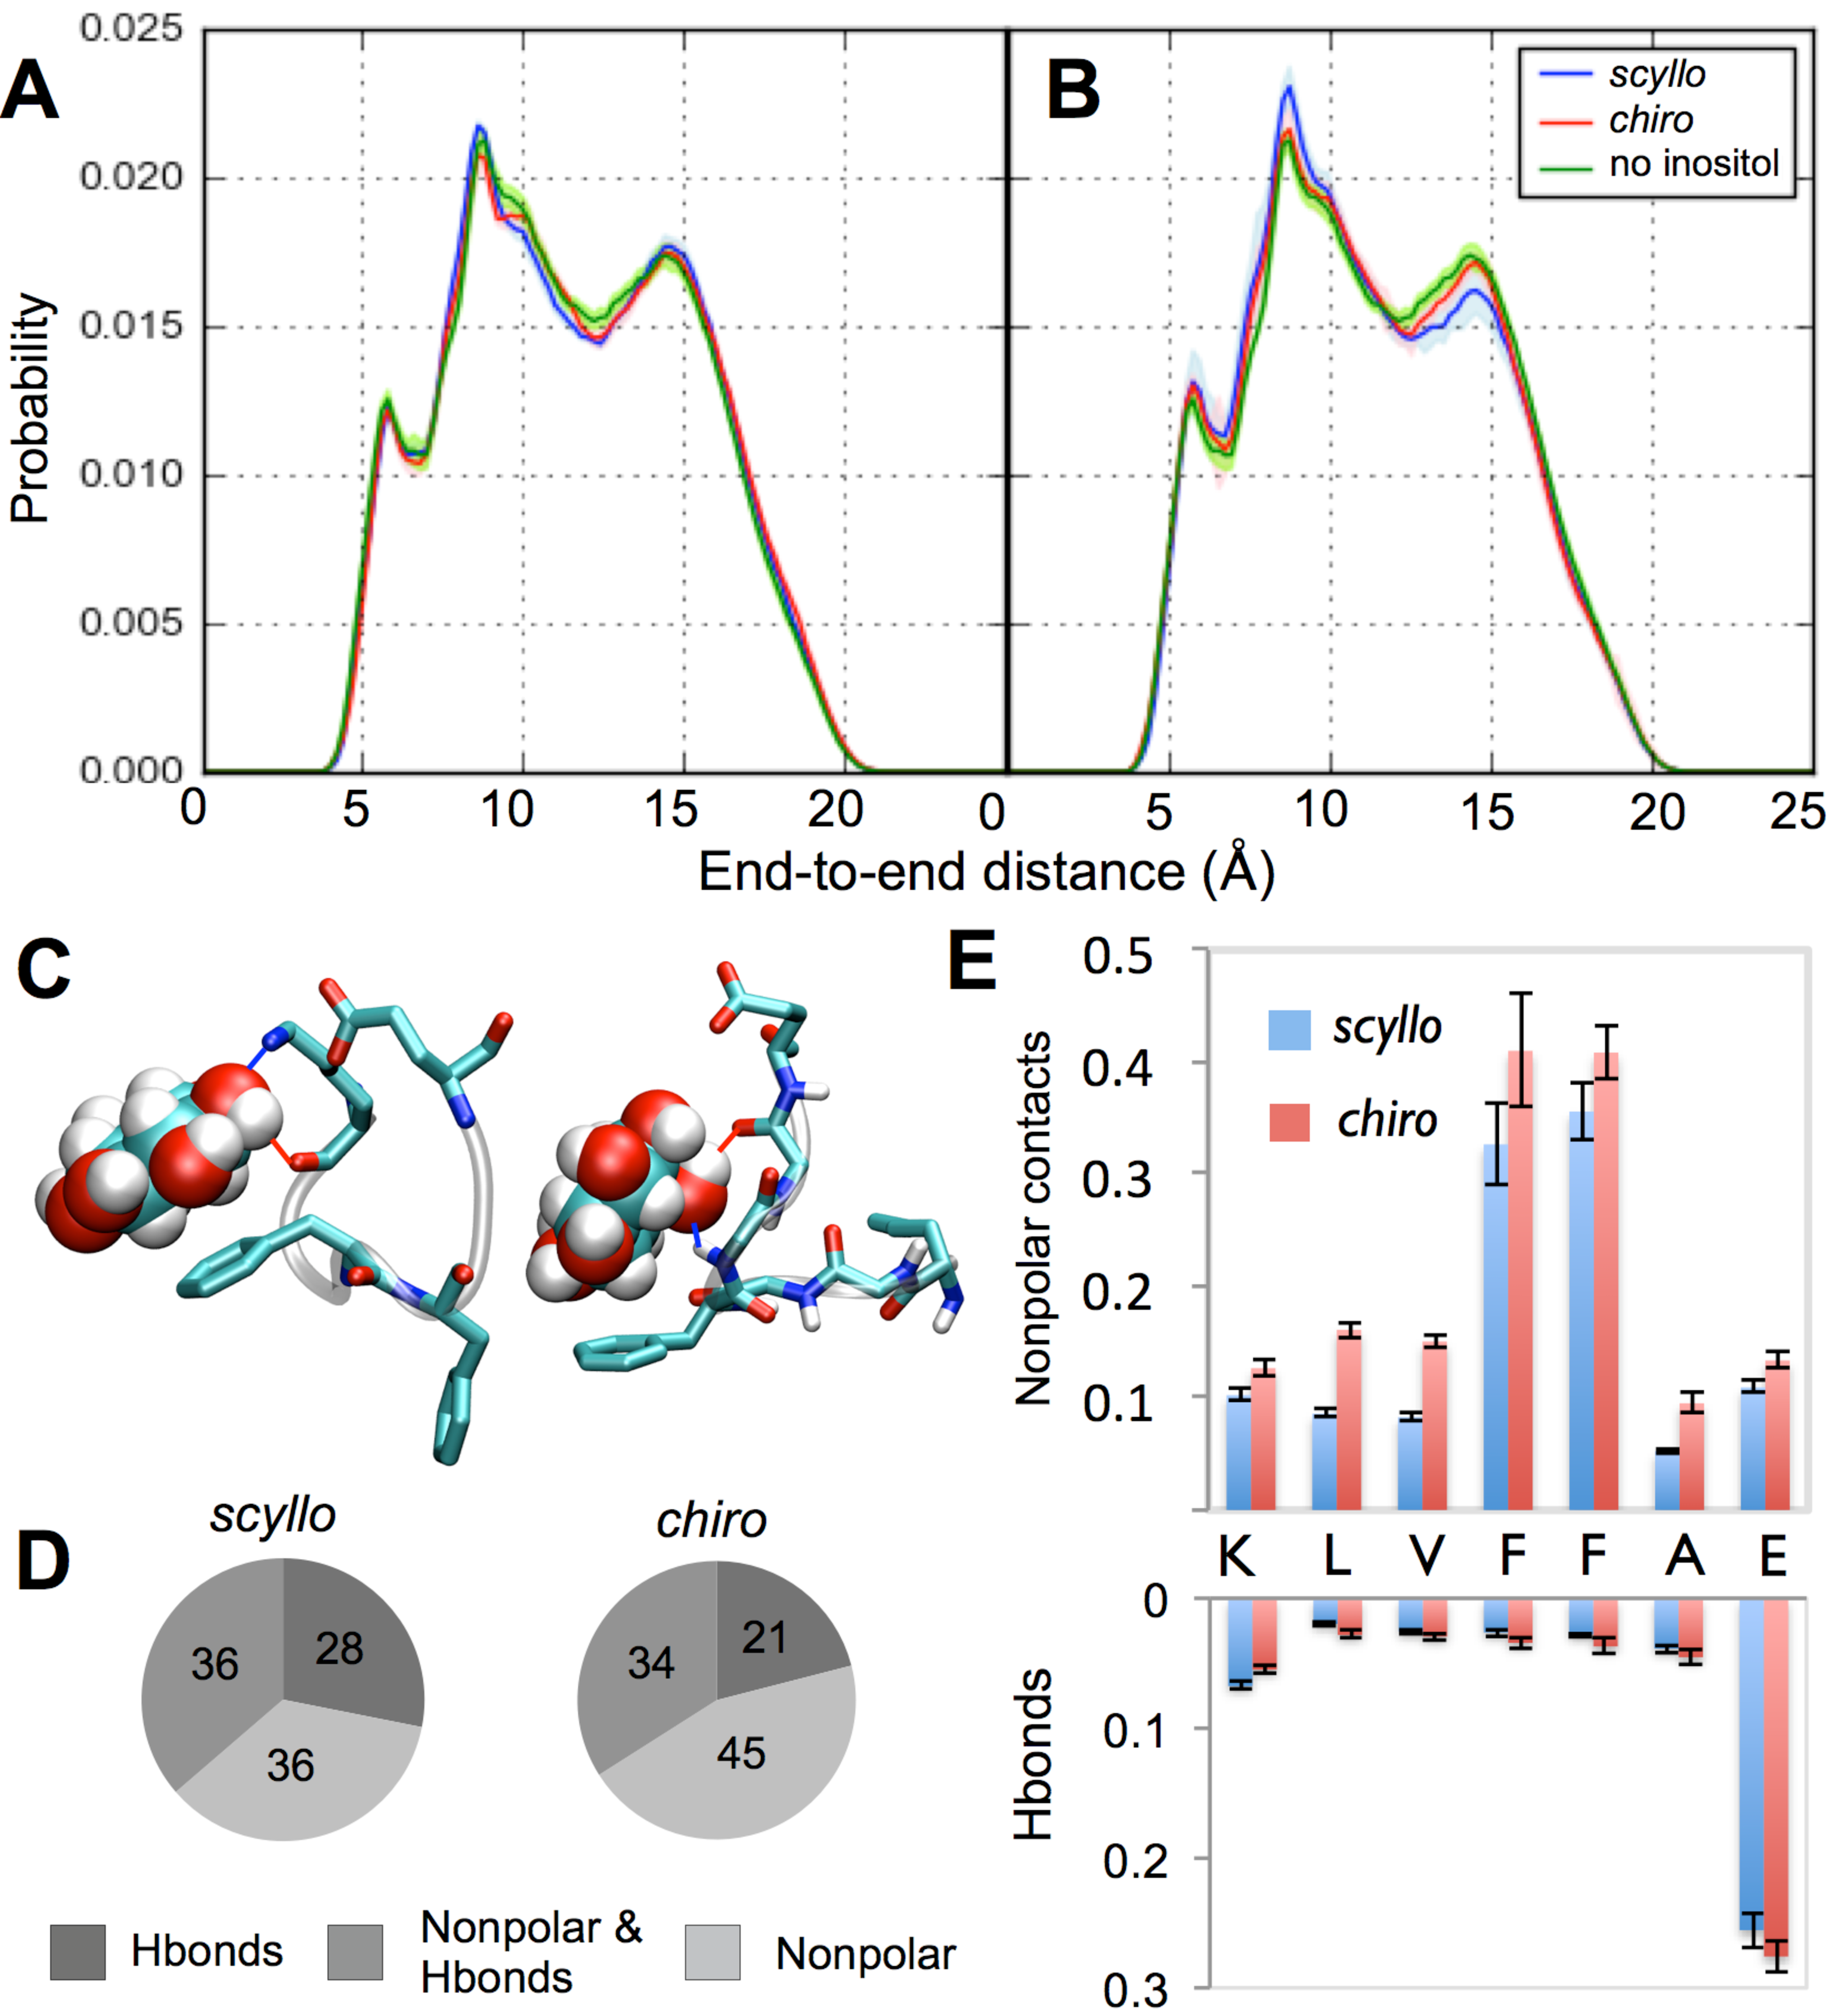
\includegraphics[width=14.6cm]{figures/results2/inos2_figures_monomers_revised.pdf}
\caption[Binding of inositol to an A$\beta$(16-22) monomer]{Binding of inositol to an A$\beta$(16-22) monomer.  End-to-end probability distribution of A$\beta$(16-22) successively in pure water and in presence of \emph{scyllo}- and \emph{chiro}-inositol at inositol:peptide molar ratios of (A) 2:1 and (B) 15:1.  (C) Representative snapshots of the different binding modes of \emph{scyllo}- (left) and \emph{chiro}-inositol (right)  to the peptide monomer. Hydrogen bonds between inositol and backbone NH (blue) and CO (red) groups are shown as solid lines. (D) Percent of bound inositol molecules in contact with nonpolar and polar groups at an inositol:peptide molar ratio of 15:1. (E) Time-averaged number of nonpolar contacts (top), and hydrogen bonds (bottom) made by inositol  (at a molar ratio of 15:1) to each residue.}
\label{fig:monomers}
\end{figure}

Independent of the presence of inositol, A$\beta$(16-22) is a disordered peptide in solution (Figure~\ref{fig:monomers}A,B) and is able to adopt both collapsed and extended states over the time scales of our simulation. The conformational equilibrium of A$\beta$(16-22), as measured by peptide end-to-end distance distributions, was unaffected by the presence of inositol at both inositol:peptide molar ratios considered (Figure~\ref{fig:monomers}A,B). The three peaks correspond to different intramolecular hydrogen-bonding arrangements (see Figures~\ref{fig:SI-monomersEedByHbonds} and \ref{fig:SI-monomersConformations} in the Supporting Information).

Inositol molecules bound weakly and reversibly to the monomer of A$\beta$(16-22). Representative examples of \emph{scyllo}- and \emph{chiro}-inositol binding are depicted in Figure~\ref{fig:monomers}C. Dissociation constants $K_{eq}$(\emph{scyllo}) = 127 $\pm$ 3 mM, $K_{eq}$(\emph{chiro}) = 104 $\pm$ 1 mM were obtained at a molar ratio of 2:1, and $K_{eq}$(\emph{scyllo}) = 120 $\pm$ 2 mM, $K_{eq}$(\emph{chiro}) = 93 $\pm$ 2 mM at a molar ratio of 15:1. Increasing the molar ratio of inositol:peptide by more than 7-fold  did not decrease the $K_{eq}$ significantly, suggesting that inositol does not bind cooperatively to the peptide monomer.
% There is very little difference in Keq between the two ratios .. is this for real ???

% Nonpolar binding
Nonpolar contacts played a significant role in inositol binding, with \emph{chiro}-inositol more likely than \emph{scyllo}-inositol to form nonpolar contacts: as shown in Figure~{\ref{fig:monomers}}D, $\sim$36\% of bound \emph{scyllo}- vs $\sim$45\% of \emph{chiro}-inositol molecules formed nonpolar contacts with the monomer. Both stereoisomers were preferentially bound to the nonpolar group of Phe over the nonpolar groups of the other residues (Figure~\ref{fig:monomers}E).

% Inositol stacking with Phe
To characterize the binding geometry of inositol to Phe in detail, we performed simulations of a Phe dipeptide in the presence of \emph{scyllo}- or \emph{chiro}-inositol. Specifically, \emph{scyllo}- but not \emph{chiro}-inositol displays a face-to-face stacking mode with the aromatic side chain of Phe (Figure~\ref{fig:monomers_glu_phe}C). This mode has an approximate binding free energy of $-$0.5 kcal/mol and appears on the potential of mean force (PMF) for \emph{scyllo}-inositol as a free energy minimum at a distance between the center of inositol and phenyl rings, $r$ = 0.45 nm, and an angle between the planes of the rings, $\theta$ = 12$\degreesymb$

%(Figure~\ref{fig:monomers_glu_phe}D, left panel). By contrast, this stacked binding mode was not observed for \emph{chiro}-inositol, which lacks planar nonpolar faces because of its adjacent axial hydroxyl groups (Figure~\ref{fig:monomers_glu_phe}D, right panel). 

% Hydrogen bonding
% Do I need some sort of transition here?
\emph{scyllo}-Inositol is more likely than \emph{chiro}-inositol to bind via hydrogen-bonding interactions: $\sim$28\% of bound \emph{scyllo}-inositol versus $\sim$21\% of bound \emph{chiro}-inositol molecules formed at least one hydrogen bond with the monomer. Inositol bound not only to the peptidic backbone of A$\beta$(16-22) but also to the charged side chains of glutamic acid (Glu) and lysine (Lys) residues. Both stereoisomers of inositol display similar hydrogen-bonding propensities to each of the residues in the peptide. % Does it make sense that scyllo and chiro have similar binding propensities, but that there is a smaller population of hbonds-bound-only chiro-inositols?
Inositol molecules bound most favorably to Glu, where their interaction was dominated by hydrogen bonding to the carboxylate group (Figure~\ref{fig:monomers}E). Both nonpolar and hydrogen bonding propensities were independent of molar ratio (Figure~{\ref{fig:monomers}} and Figure~{\ref{fig:SI-monomersBinding}} in the Supporting Information). Furthermore, we found an equal fraction of monodentate and bidentate binding (Figure~\ref{fig:monomers_glu_phe}A) to the carboxylate group of Glu (Figure~\ref{fig:monomers_glu_phe}B). In contrast, less than 1\% of inositol molecules bound to Lys involved multiple hydrogen bonds to the ammonium group (Figure~\ref{fig:monomers_glu_phe}B).

\begin{figure}
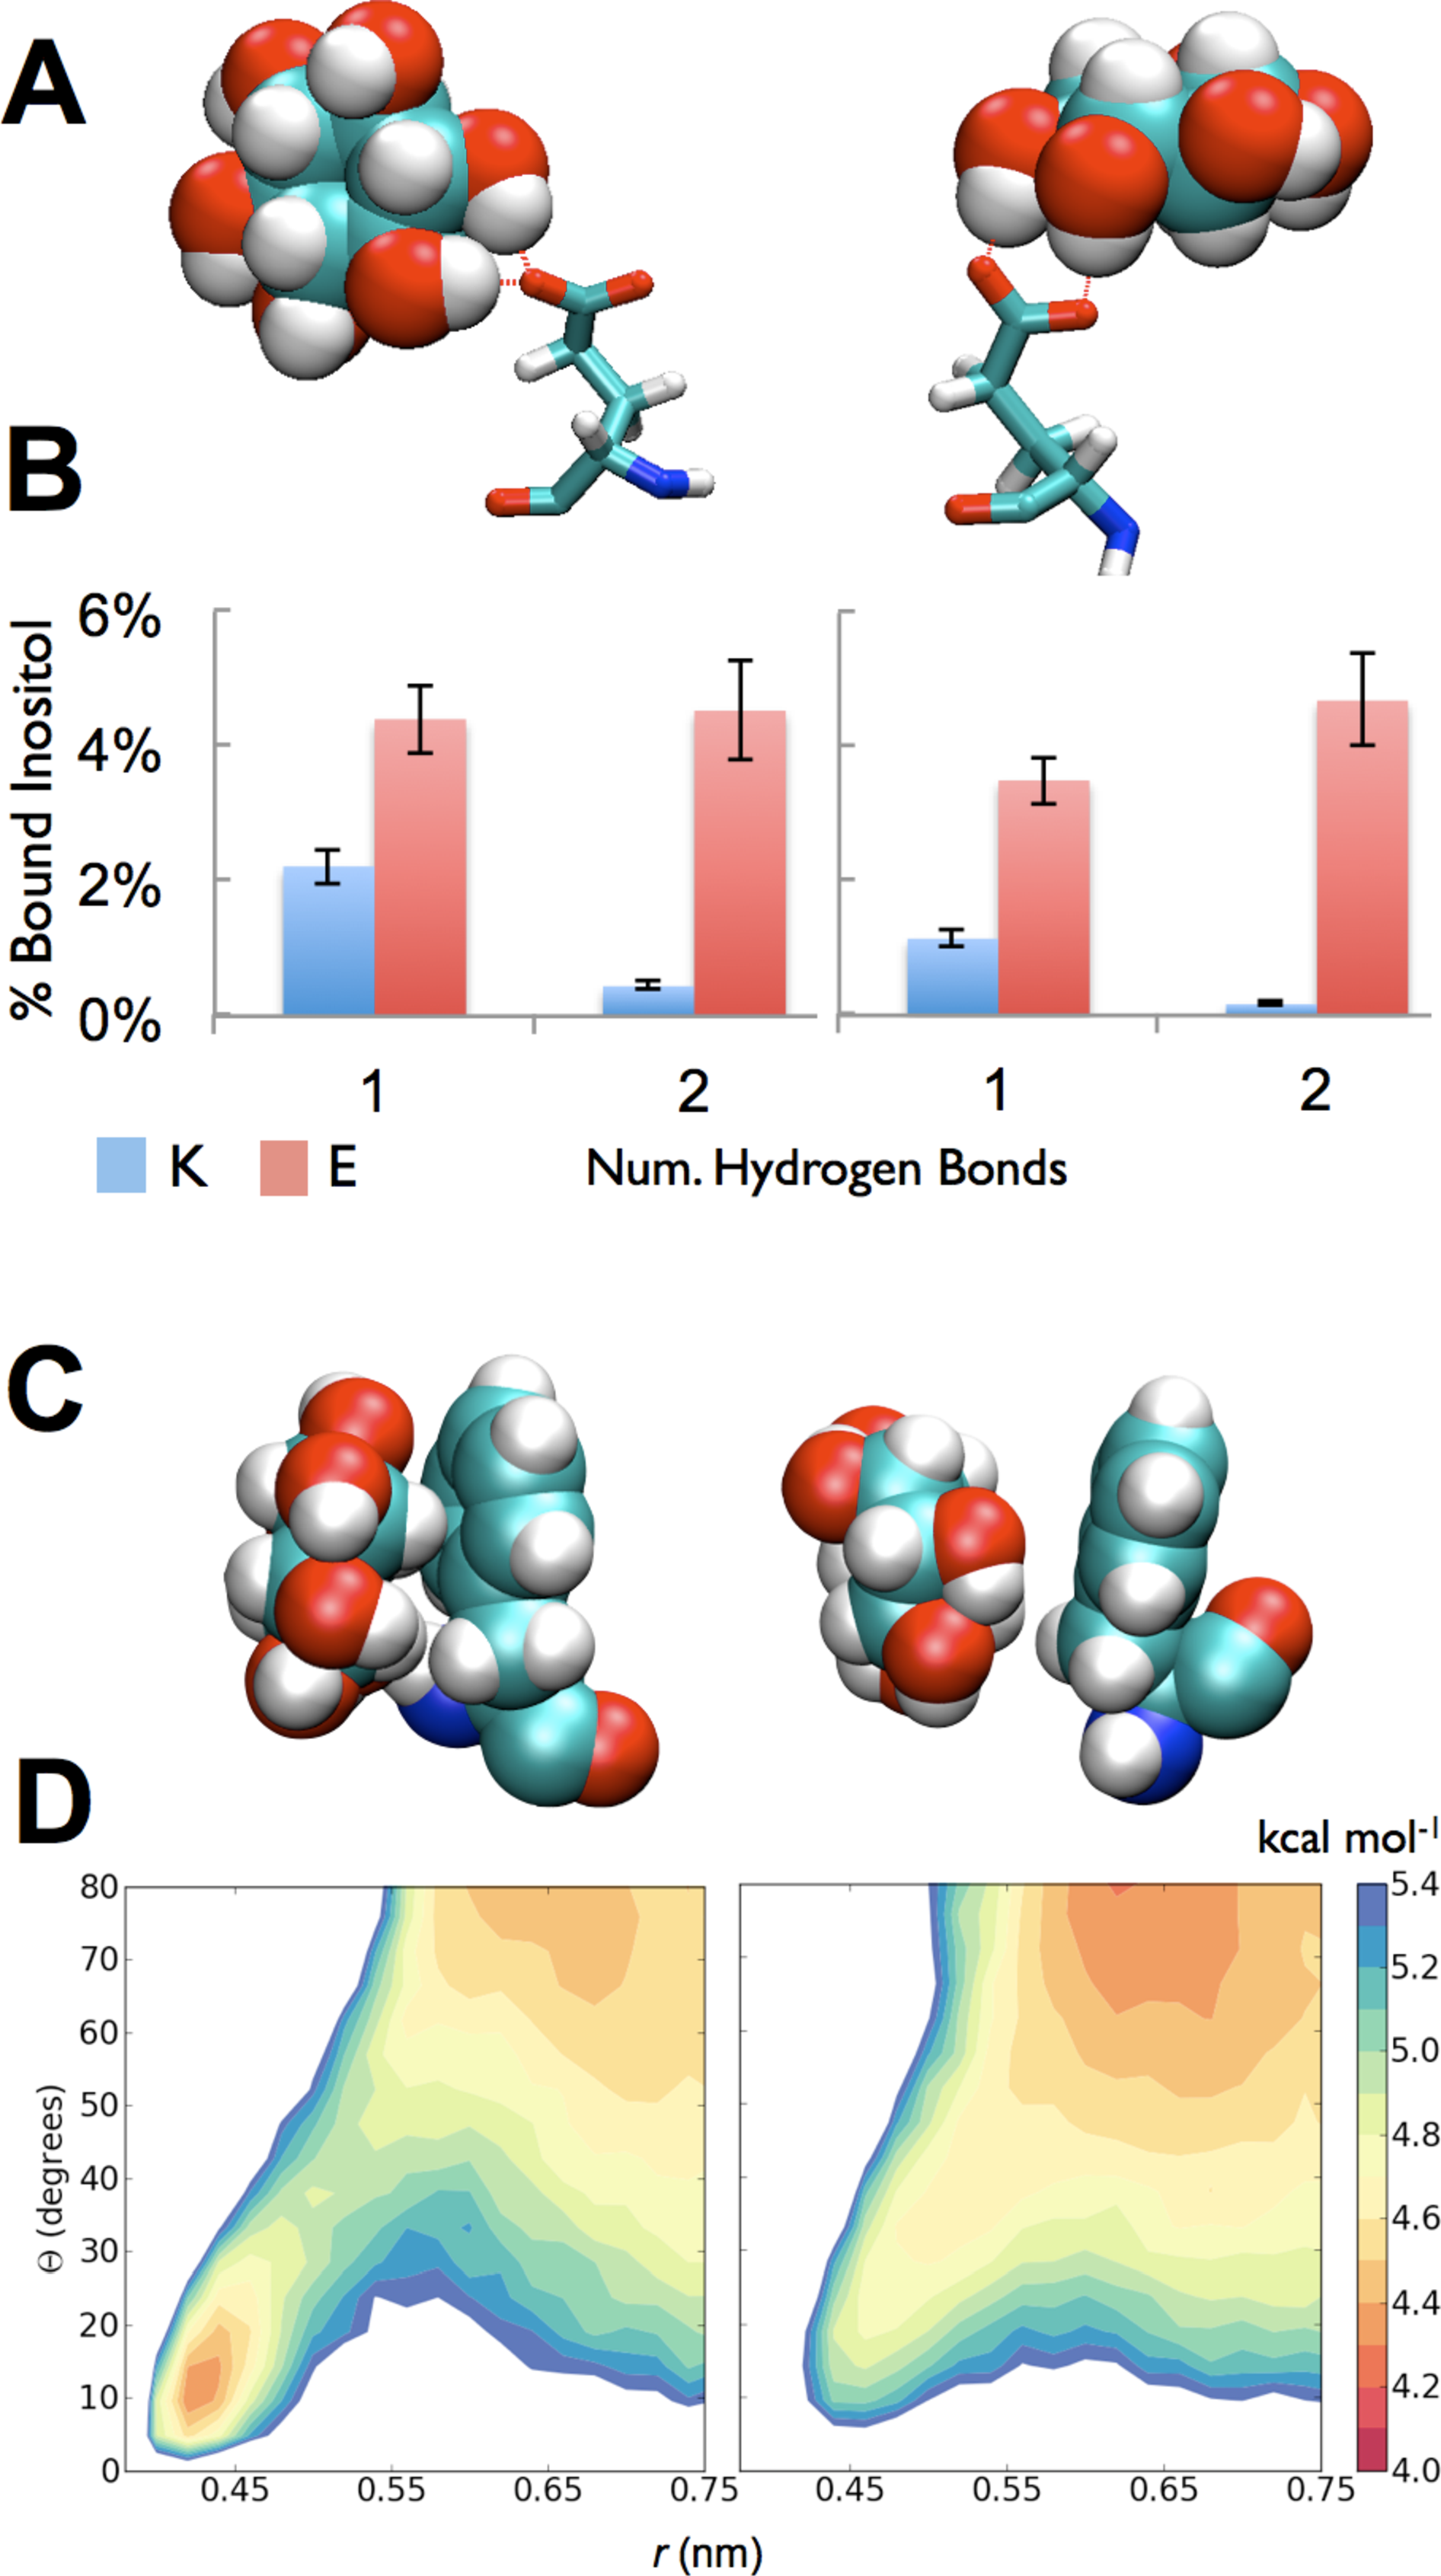
\includegraphics[width=3.185in]{figures/results2/inos2_figures_monomer_residues_pmf_color.pdf}
\caption[Binding of inositol to Glu and Phe dipeptides]{Binding of inositol to Glu and Phe dipeptides. Data for \emph{scyllo}- and \emph{chiro}-inositol are shown on the left and right panels, respectively. (A) Examples of snapshots of inositol bound to the carboxylate group of Glu. (B) Comparisons of the probability of inositol hydrogen bonding to the side chains of Lys and Glu. (C) Examples of nonpolar association between Phe and inositol. (D) Potential of mean force (PMF) of inositol with the phenyl ring of Phe relating $r$, the distance between the centers of geometry of the phenyl and inositol rings, to $\theta$, the planar angle between the rings. Contours are drawn at 0.1 kcal$\cdot$mol$^{-1}$ intervals. Face-to-face stacking for \emph{scyllo}-inositol appears on the PMF at $r=0.45$ nm and $\theta=12\degreesymb$.}
\label{fig:monomers_glu_phe}
\end{figure}

%Furthermore, consistent with our previous study of (GA)$_4$, stereochemistry appears to modulate nonpolar binding, but not hydrogen bonding: \emph{scyllo}-inositol was found to bind preferentially to nonpolar groups on phenylalanine and glutamate over the other aliphatic nonpolar residues (Leu, Val and Ala) (Figure~\ref{fig:monomers}E). By contrast, \emph{chiro}-inositol made nonpolar contacts to Phe18, Phe19 and Glu22 with the same probability as with Ala21 (Figure~\ref{fig:monomers}E).

% \sethlcolor{yellow}\hl{Furthermore, of the population of scyllo-inositols bound to Phe via nonpolar contacts, XXX\% of  were bound in the stacked binding mode at a ratio of 15:1, and 7\% at a ratio of 2:1. SHOULD STACKING RESULTS JUST BE MENTIONED IN THE DISCUSSION?}

% I determined the 58% by computing the fraction of all inositols that were stacked divided by the total number of inositols bound to Phe over all frames -- this isn't quite correct because the bound Phes were only counted when the COM (phe, inos) < 0.45 nm
% I need to join this data with the data on the number of nonpolar contacts between phe and inositol

% Note that binding constants similar between low and high molar ratios for monomers once I've switched to the atomic-based contact pairs ... but the difference in kd was more dramatic under the other criteria ... could this mean that there are more stacking interactions at higher molar ratios?
%binding mode of scyllo to the monomer. Given a bound scyllo-inositol molecule to phe (it doesn't really make sense otherwise), it is predominantly bound by XXX, where X\% of time it is  stacking and 100 - X not stacked}.

\subsection{Disordered Oligomer}

To probe the effect of inositol on the early aggregation stages of A$\beta$(16-22), we performed multiple sets of independent MD simulations with four initially disperse A$\beta$(16-22) monomers with inositol:peptide molar ratios of 2:4, 15:4, and 45:4, corresponding to inositol concentrations of 52 mM, 70 mM, and 209 mM, respectively (see Table~\ref{tbl:simulations}). In each of our simulation studies, the peptides spontaneously aggregated with one another over the course of approximately 40 ns, through both hydrogen bonding and nonpolar contacts, to form a disordered oligomer (Figure~\ref{fig:disordered}A). A significant fraction of the residues in the aggregate was in the coil conformation, with only a small fraction of $\beta$-sheet residues occurring in some of the 180-ns simulations (Ffigures/results2igure~\ref{fig:disordered}B). Importantly, the distribution of the overall secondary structure of the oligomer was not affected by the presence of inositol, regardless of inositol:peptide molar ratio and inositol concentration (Figure~\ref{fig:disordered}B).

\begin{figure}figures/results2
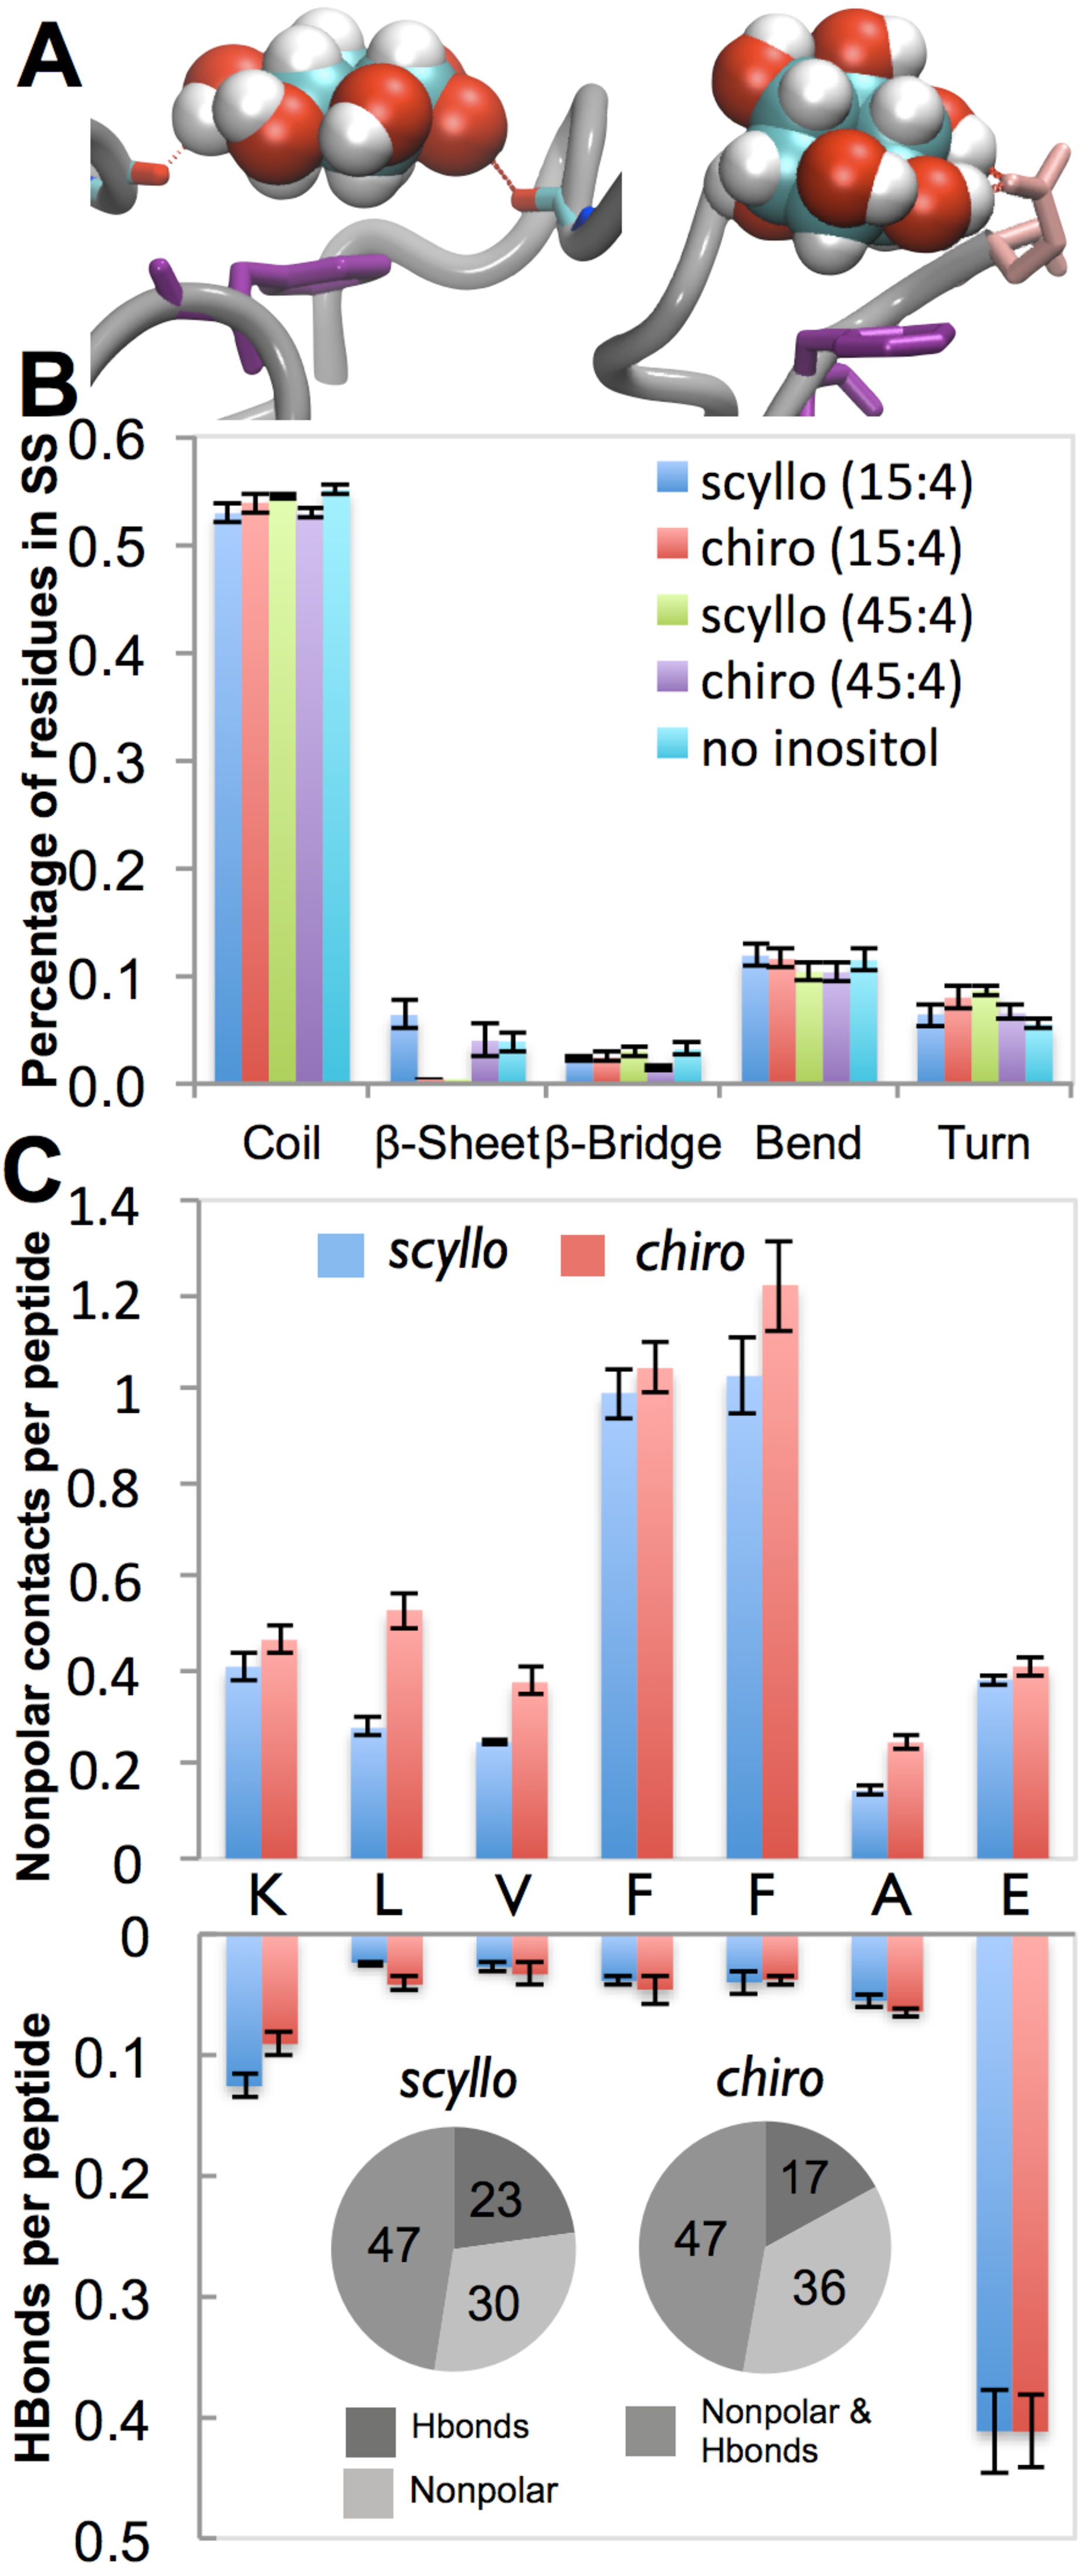
\includegraphics[width=7.96cm]{figures/results2/inos2_figures_disordered_revised.pdf}
\caption[Binding of inositol to a disordered oligomer of A$\beta$(16-22)]{Binding of inositol to a disordered oligomer of A$\beta$(16-22).  (A) Example snapshots of \emph{scyllo}- (left) and \emph{chiro}-inositol (right) involving both nonpolar contacts and hydrogen bonding. (B) Fraction of residues in coil, $\beta$-sheet/bridge, bend, and turn conformations as classified by the DSSP algorithm. (C) Time-averaged number of nonpolar contacts (top) and hydrogen bonds (bottom) made by inositol to each residue (per peptide). Inset: Percent of inositol molecules bound to nonpolar and polar groups of the peptide oligomer at an inositol:peptide molar ratio of 45:4 (inositol concentration of 209 mM).}
\label{fig:disordered}
\end{figure}

We further characterized the molecular organization of the aggregate by quantifying peptide inter- and intramolecular hydrogen-bonding and nonpolar contacts as measures of the extent of aggregation.  Hydrophobic packing was not affected by the presence of inositol: the equilibrium number of inter-peptide hydrophobic contacts formed per peptide remained approximately 15 regardless of the molar ratio (Figure~\ref{fig:SI-disorderedNumContacts} in the Supporting Information). The average number of intermolecular peptide-peptide hydrogen bonds per chain was approximately the same as the number of intramolecular hydrogen bonds (1.5 vs 1) (Figure~\ref{fig:SI-disorderedNumContacts} in the Supporting Information). Overall, the presence of inositol had no significant effect on the aggregation kinetics or on the morphology of A$\beta$(16-22) oligomers as measured by intermolecular and intramolecular contacts (Figures~\ref{fig:SI-disorderedContactsTS} and \ref{fig:SI-disorderedCluster} in the Supporting Information).

\begin{table}\footnotesize
  \vspace{10pt}
  \caption{Summary of equilibrium constants (K$_{eq}$) and number of reversible binding events (N$_{binding}$)}

  \label{tbl:bindingConstants}
  \begin{minipage}{15cm}
    \renewcommand{\thefootnote}{\thempfootnote}
    \renewcommand{\footnoterule}{}
    % \centering
      \begin{center}
    \begin{tabular}{| l | *{6}{ c |}}
       \hline
         System & Molar ratio\footnote{Inositol:peptide molar ratios} & K$_{eq,scyllo}$\footnote{K$_{eq}$ is in units of mM. The standard error is shown within parentheses.} & K$_{eq,chiro}$\footnotemark[\value{mpfootnote}]  & N$_{binding,scyllo}$\footnote{N$_{binding}$ is the total number of reversible inositol binding events.} & N$_{binding,chiro}$\footnotemark[\value{mpfootnote}] \\
         \hline
         \hline
         Monomer & 2:1 & 127 (3) & 104 (1)  &  150991 & 185454 \\ % & 104 \\ 
          	       & 15:1 & 120 (2) & 90 (2)  & 186948 & 250922  \\ % & 90 \\ 
	\hline
         Disordered oligomer & 2:4 & 28 (4) & 16 (2) &  21882 & 24584 \\ % & 23 \\ 
          			       & 15:4 & 18 (2) & 11(1) & 78483 & 102351 \\ % & - \\ 
				       % & 45:4 & 1.6 (0.4) & 1.9 (0.9) & 15501 & 18101 \\ 
	\hline
         $\beta$-oligomer & 4:16 & 15 (2) & 11 (2) & 20381 & 24616 \\ % & 6\\
         				  & 64:16 &  0.5 (0.3) & 0.18 (0.11) & 50135 & 56842 \\ % & -\\
         \hline
     \end{tabular}   
  \end{center}
  \end{minipage}
  \centering
  \end{table}

The equilibrium constant ($K_{eq}$) of inositol with the disordered oligomer at molar ratios 2:4 and 15:4 ranged from 10 to 30 mM (see Table~\ref{tbl:bindingConstants}).
% Although these numbers are much smaller than $K_{eq}$ of the monomer, they become comparable when normalized by the number of peptides in the system, $K_{eq}$ (oligomer) $\times$ 4 = 170 mM = $K_{eq}$(monomer), indicating that inositol does not bind small oligomeric aggregates cooperatively. 
% Based on the updated analysis and Keqs -- Binding constants do not indicate cooperative binding at low molar ratios (eg. 2:4 and 2:1), however, at higher molar ratios, a nonlinear decrease in binding constants was observed.  
% I think mention of cooperativity should be entirely moved to the discussion section ...
Similar proportions of bound inositol to nonpolar and polar groups were found at both lower and higher molar ratios (Figure~{\ref{tbl:SI-disorderedBindingMode}} in the Supporting Information). Consistent with our results for the monomer, \emph{chiro}-inositol was more likely than \emph{scyllo}-inositol to bind disordered oligomers exclusively via nonpolar contacts: $\sim$26\% and $\sim$36\% for \emph{scyllo}- and \emph{chiro}-inositol, respectively (Figure~\ref{fig:disordered}C inset and Table~\ref{tbl:SI-disorderedBindingMode}).  
%By contrast, both \emph{scyllo}- and \emph{chiro}-inositol have similar hydrogen bonding propensities (Figure~{\ref{fig:disordered}}C). 
Inversely, \emph{scyllo}-inositol was more likely to bind by hydrogen bonding only ($\sim$23\% vs. $\sim$17\%). Although the number of hydrogen bonds formed along the peptide sequence were independent of inositol concentration (Figure~\ref{fig:disordered}, \ref{fig:SI-disorderedBinding}), the number of nonpolar contacts per peptide approximately doubled upon increasing inositol concentration from 70 to 209 mM.

\subsection{$\beta$-oligomer}

\begin{figure}
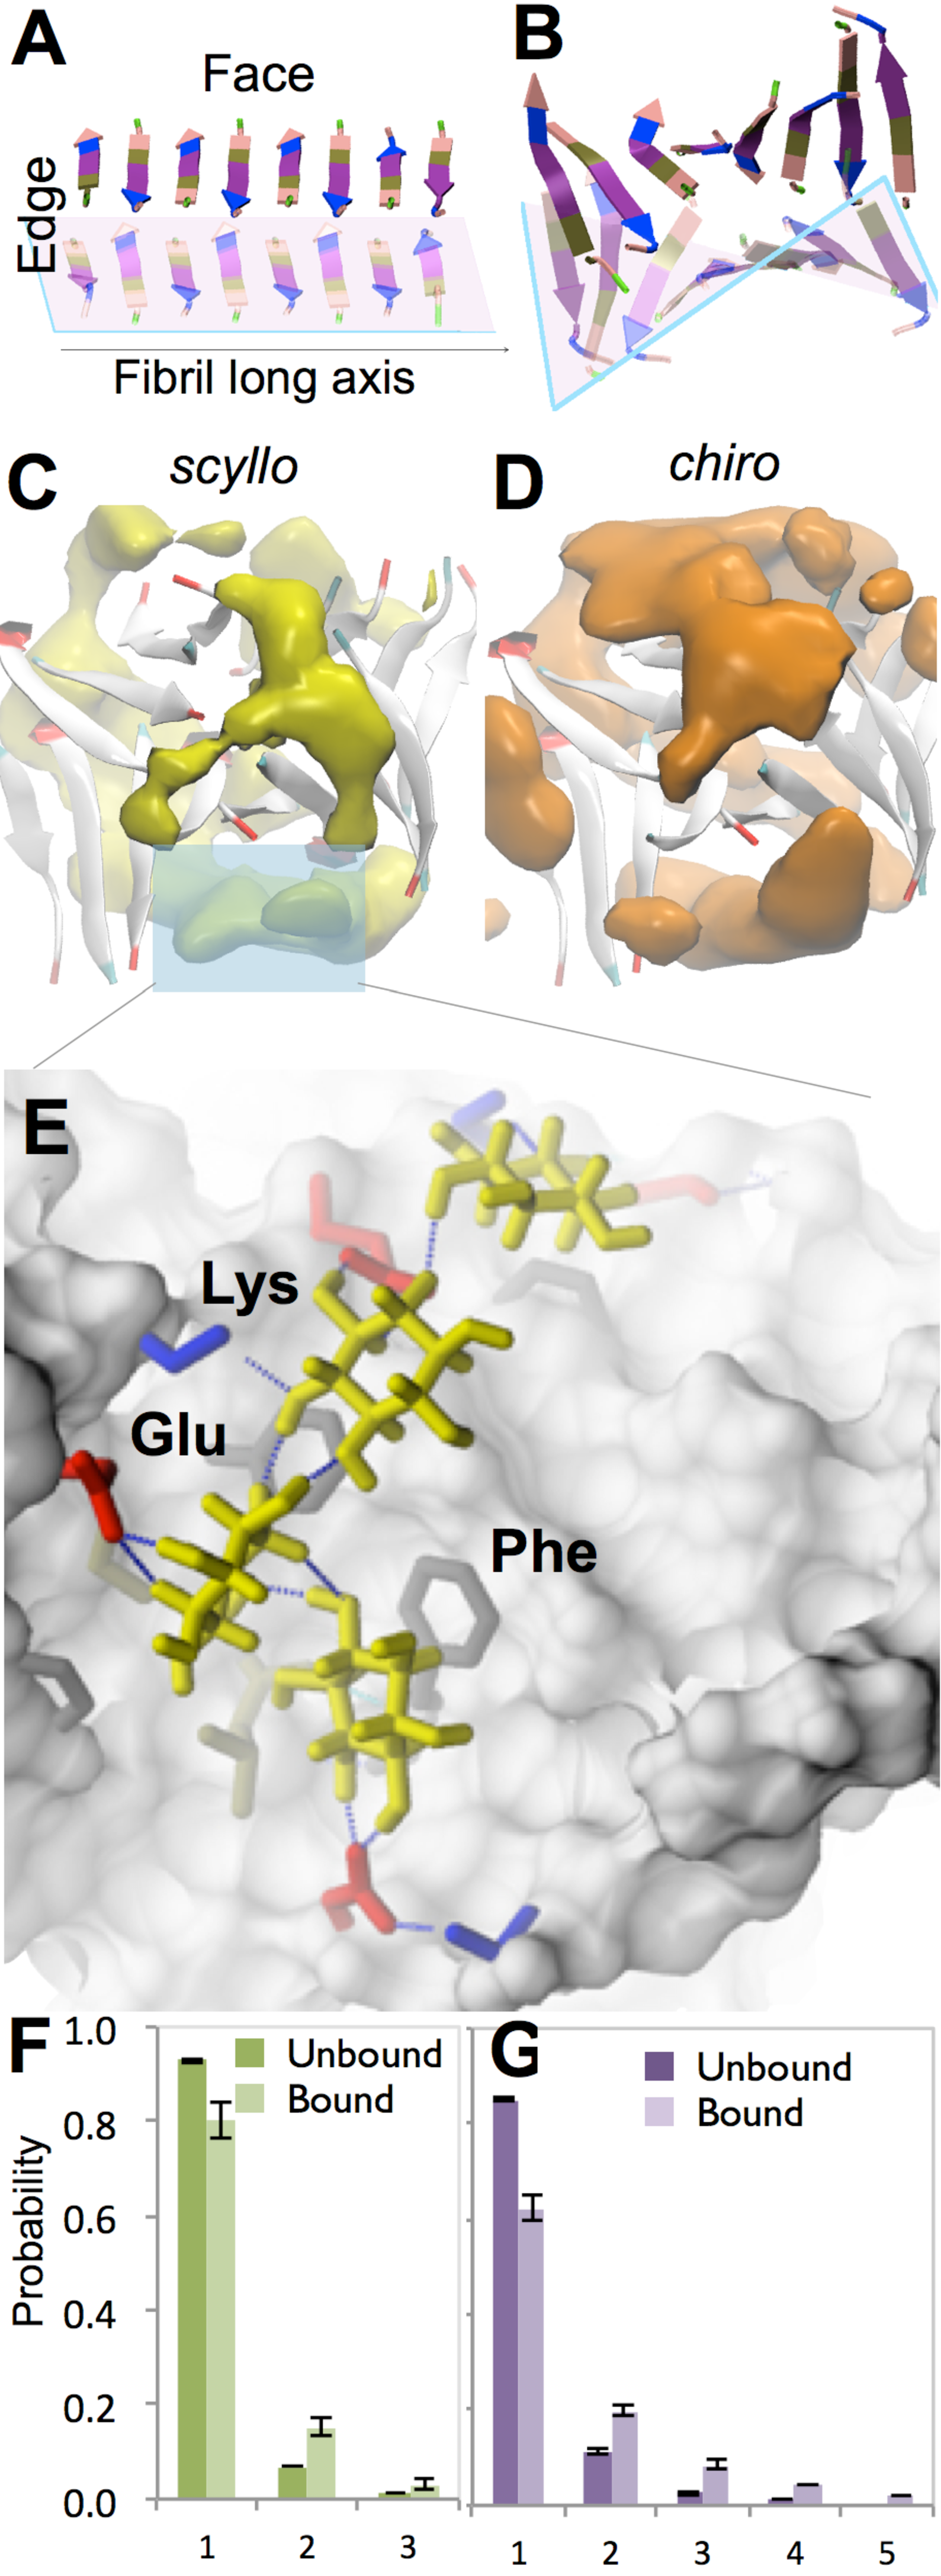
\includegraphics[width=8.1cm]{figures/results2/inos2_figures_beta.pdf}
\end{figure}
\begin{figure}[t!]
\caption[Inositol binding to a $\beta$-oligomer of A$\beta$16-22]{Inositol binding to a $\beta$-oligomer of A$\beta$16-22. Schematic depiction of $\beta$-oligomer twisting: (A) the initial rectangular dual-stacked $\beta$-sheet, evolved into (B) a twisted morphology. Spatial probability density maps of (C) \emph{scyllo}-inositol and (D) \emph{chiro}-inositol are shown in yellow and orange, respectively.  Concentration of inositol is 208 mM and surfaces shown correspond to 7\% inositol occupancy. (E) An example of cooperatively-bound \emph{scyllo}-inositol molecules (yellow) at the surface of the $\beta$-oligomer (grey). Size distribution of bound and unbound clusters of \emph{scyllo}-inositol with the $\beta$-oligomer at inositol concentrations of (F) 62 mM and (G) 208 mM.}
\label{fig:beta}
\end{figure}

Finally, we examine the binding of inositol to an ordered protofibrillar-like aggregate henceforth referred to as the $\beta$-oligomer. In the absence of inositol, rectangularly-stacked sheets (Figures~\ref{fig:SI-betaInitialModel}A-B) spontaneously evolved into a twisted $\beta$-sheet structure with significant inter-strand twisting along the long-axis of the fibril and an inter-sheet twist (Figures~\ref{fig:beta}A-B). The resulting structure has an average inter-strand twist angle of approximately 25$\degreesymb$ for the top sheet and 15$\degreesymb$ for the bottom sheet. Furthermore, the $\beta$-oligomer is comprised of two faces and four edges (Figure~\ref{fig:SI-betaInitialModel}), each of which contains a shallow hydrophobic groove surrounded by polar or charged groups.  In particular, the grooves on the faces are formed by solvent-exposed Phe, Val, and Ala residues and are surrounded on either side by charged side chains of Lys and Glu (Figure~\ref{fig:SI-betaInitialModel}C).

The spatial probability densities of bound inositol depicted in Figures~\ref{fig:beta}C-D show that inositol predominantly binds at the faces of the $\beta$-oligomer. Both stereoisomers have similar affinities with $K_{eq}=$ 15 $\pm$ 2 mM and 11 $\pm$ 2 mM for \emph{scyllo}- and \emph{chiro}-inositol, respectively, at a concentration of 37 mM (inositol:peptide molar ratio of 4:16), and $K_{eq}=$ 0.5 $\pm$ 0.3 mM and 0.18 $\pm$ 0.11 mM at a concentration of 62 mM (molar ratio of 64:16) (Table~\ref{tbl:bindingConstants}).   
% Moving this sentence down to discussion -- Furthermore, $K_{eq}$'s of both stereoisomers decreased significantly (corresponding to an increase in binding) with an increase of inositol:peptide molar ratio, suggesting that the inositols may bind $\beta$-oligomers cooperatively.

% Results that are independent of concentration
% Also note that I'm stating the results without qualifying the molar ratio or concentration ... I should have a statement either saying they are the same at first, then stating the specifics.
Consistent with the binding densities depicted in Figure~\ref{fig:beta}, inositol molecules display the highest binding propensity to the nonpolar groups of Phe and Lys and the charged groups of Lys and Glu, all of which are located on the faces of the $\beta$-oligomer (Figure~\ref{fig:SI-betaInitialModel}C). Inositol molecules did not penetrate the $\beta$-sheet core of the oligomer: the fraction of hydrogen bonds to each residue depicted in Figure~\ref{fig:beta_residue_binding} (bottom panel) show that, relative to side chains, little or no hydrogen bonds were made with the backbone of residues Leu, Val, Phe, and Ala. Although inositol molecules sometimes intercalated between $\beta$-strands, these rare events did not lead to the disaggregation of the preformed $\beta$-oligomer in any of our simulations.

\begin{figure}
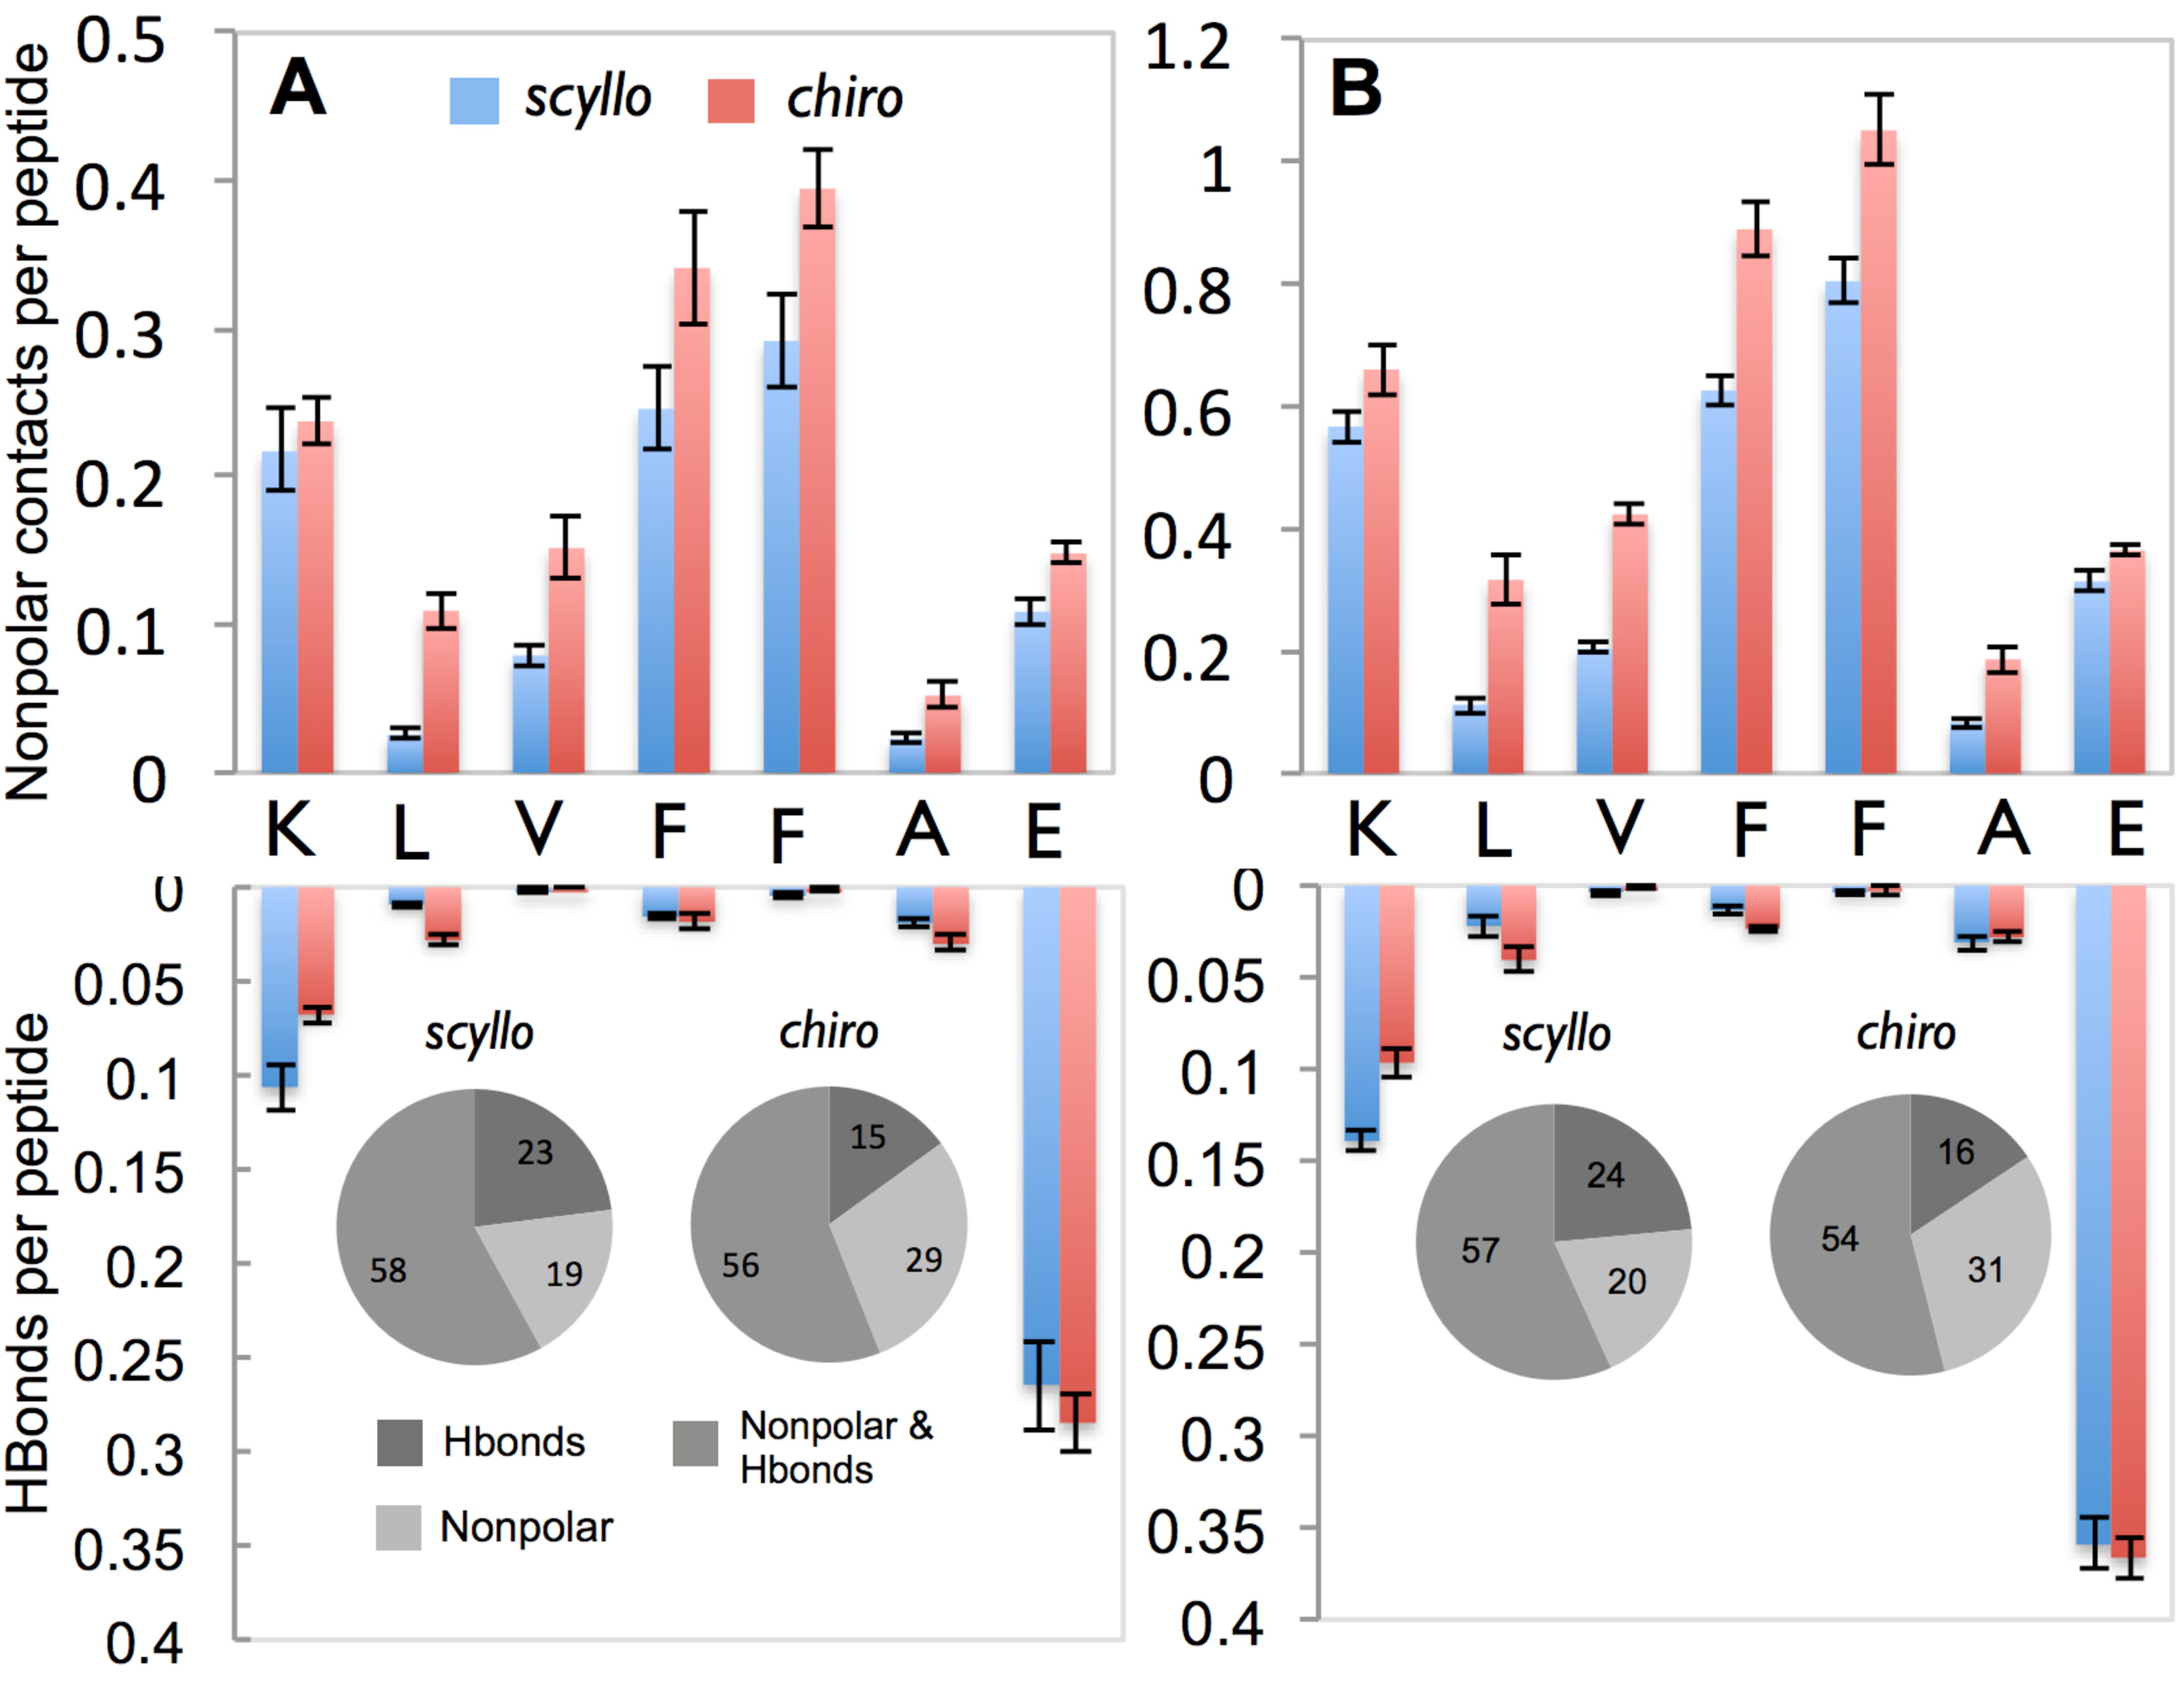
\includegraphics[width=15cm]{figures/results2/inos2_figures_beta_residues_revised.pdf}
\caption[Binding propensity of inositol to nonpolar and polar groups of the $\beta$-oligomer]{Binding propensity of inositol to nonpolar and polar groups of the $\beta$-oligomer. Average number of nonpolar contacts (top) and hydrogen bonds (bottom), per peptide, made by inositol to each residue of the $\beta$-oligomer. Inset: Percent of \emph{scyllo}- and \emph{chiro}-inositol molecules bound to nonpolar and polar groups of the $\beta$-oligomer.  Inositol is present at a concentration of 62 mM in part A and 208 mM in part B.}
\label{fig:beta_residue_binding}
\end{figure}

Independently of inositol concentration, a higher fraction of \emph{scyllo}-inositol than \emph{chiro}-inositol formed hydrogen bonds with the $\beta$-oligomer (inset of Figure~\ref{fig:beta_residue_binding} and Table~\ref{tbl:SI-betaBindingMode}):  $\sim$23\% versus $\sim$15\%, respectively. Concomitantly, the fraction of \emph{chiro}-inositol molecules forming nonpolar contacts ($\sim$29\%) was higher than that of \emph{scyllo}-inositol ($\sim$19\%) (inset of Figure~\ref{fig:beta_residue_binding} and Table~\ref{tbl:SI-betaBindingMode}).

% Results which are modulated by concentration
% \sethlcolor{green}
At the higher inositol:peptide molar ratio of 64:16, bound inositol molecules were significantly more likely to be clustered than free inositol: 20\% versus 8\% (Figure~{\ref{fig:beta}}F-G) at 62 mM. Moreover, the size of bound clusters increased with concentration. Inositol molecules within a cluster were usually hydrogen bonded 
% this may not be right because they can form nonpolar contacts too
to each other via their free hydroxyl groups, while simultaneously forming hydrogen bonds and/or nonpolar contacts with the peptide.  Such a binding mode is depicted in Figure~{\ref{fig:beta}}E, where a hydrogen-bonded chain of four  \emph{scyllo}-inositol molecules occupies a shallow groove on the $\beta$-oligomer surface. % [Add additional examples of clustered binding to SI for both scyllo and chiro and reference them here]
There was no difference in distribution of cluster size between \emph{chiro}- and \emph{scyllo}-inositol.

Furthermore, the binding propensity of \emph{scyllo}- and \emph{chiro}-inositol for hydrophobic groups increased with inositol concentration (Figure~\ref{fig:beta_residue_binding}).  At lower concentrations ($\sim$30 - 60 mM), both nonpolar and hydrogen bonding propensities increased with molar ratio, suggesting that single molecules and dimers of inositol have similar binding propensities, and binding to the protofibril involves forming both nonpolar contacts and hydrogen bonds.  However, at a concentration of 208 mM, the nonpolar binding propensity of inositol increased whereas the hydrogen bonding propensity remained the same.  As a result, inositol molecules in large clusters (of size three or more) form, on average, more nonpolar contacts with the $\beta$-oligomer than their singly-bound counterparts.
% \sethlcolor{yellow}
% I took out cooperative binding modes in the description of Figure 4E because that is implying that there is cooperativity without any evidence -- this speculate/extrapolation will be left to the discussion section.

% Move the comparisons of this is modulated by stereochemistry and aggregate morphology.
% This is a result not previously observed for the monomer and disordered oligomer of A$\beta$(16-22).

% TODO ADD/Find EVIDENCE FOR KLVFFAE IMPORTANT FOR STACKING -- I could be just bullshitting here, in any case, stacking interface mediated by KLVFFAE is not the only reason why binding to this segment is useful .. LVFFA is also at the fibril core .. disrupting packing here disrupts amyloid formation of Abeta42].  \cite{Takeda:2009es} -- Caflish and Derreumaux computation evidence that 12-22 is the "aggregation interface"

% TODO Look into this further: My results are exactly consistent with the mechanism proposed by Porat for polyphenol inhibition! planar + equatorial OHs => target amyloidgenic core! Except I have data to prove it. EGCG, an effective inhibitor of Abeta42 amyloid formation, has this structure and was shown to bind fibrillar forms of Abeta42.\cite{Bieschke:2010ju}

\section{Discussion}
In the above analysis, we have systematically characterized the binding of \emph{scyllo}-inositol and its inactive stereoisomer, \emph{chiro}-inositol, with monomer and aggregates of A$\beta$(16-22). Below, we consider the implications of our findings for the activity of inositol in the A$\beta$42 amyloid aggregation pathway.

\subsection{Comparison of inositol binding to monomers and aggregates of A$\beta$(16-22)}
Consistent with our results on the binding equilibrium of inositol with model amyloidogenic peptides,\cite{Li:2012p853} both \emph{scyllo}- and \emph{chiro}-inositol bound weakly, and with similar binding constants, to the monomeric and aggregated states of A$\beta$(16-22) considered. % Should I leave this extrapolation to full-length A$\beta$ ?
However, the equilibrium constants ($K_{eq}$) computed in this study are about an order of magnitude smaller than those obtained in our previous study, namely, in the range of 0.2 - 120 mM for A$\beta$(16-22) versus 40 - 1000 mM for a model peptide of similar length, $(GA)_4$.\cite{Li:2012p853} Because all observed binding sites and modes are accounted for in the calculation of $K_{eq}$ in our study, this quantity should be interpreted as an estimate of the binding avidity rather than the binding affinity of inositol.  This decrease in $K_{eq}$, and hence, an increase in binding avidity, is due to the presence of sequence-specific binding sites and modes in A$\beta(16-22)$.

Both \emph{scyllo}- and \emph{chiro}-inositol bound most weakly to monomers, with $K_{eq}=$ 120 $\pm$ 2 mM and 90 $\pm$ 2 mM, respectively, at the highest molar ratio (Table~\ref{tbl:bindingConstants}). Because inositol binding to the peptide monomer is not cooperative, a predicted $K_{eq}$ of monomeric A$\beta$42 can be obtained by linearly scaling the $K_{eq}$ of inositol for monomeric A$\beta$(16-22) with the ratio of peptide lengths of A$\beta$(16-22) to A$\beta$(1-42).  On the basis of the value of $K_{eq}$ of inositol at the highest molar ratio, this value would be 120 mM/6 = 20 mM, which is an order of magnitude higher than the concentration (1 mM) at which inhibition was observed \emph{in vitro}.\cite{McLaurin:2000p64}  Moreover, our results indicate that the conformational equilibrium of monomeric A$\beta$(16-22) is not displaced in the presence of inositol (Figure~\ref{fig:monomers}A). Taken together, these results suggest that inositol is unlikely to act as a drug by binding to and displacing the conformational equilibrium of monomers of A$\beta$42.

Likewise, inositol bound only weakly to small disordered oligomers, with $K_{eq}$ $\sim$10 - 30 mM at a concentration of 70 mM for both \emph{scyllo}- and \emph{chiro}-inositol (Table~\ref{tbl:bindingConstants}). Independently of the presence of inositol,  A$\beta$(16-22) peptides formed amorphous aggregates with only a small amount of secondary structure. These aggregates predominantly involved intermolecular nonpolar contacts (Figure~\ref{fig:SI-disorderedContactsTS}), indicating that hydrophobic association is the primary driving force for the self-assembly of A$\beta$(16-22) peptides in solution. Inositol molecules were found to bind both monomers and small oligomers of A$\beta$(16-22) predominantly via nonpolar interactions (Figures~{\ref{fig:monomers}} and {\ref{fig:disordered}}),  suggesting that they may disrupt the hydrophobic association of nonpolar groups. However, due to weak binding, we speculate that inositol is unlikely to prevent early oligomer formation in the A$\beta$42 fibrillation pathway by binding to A$\beta$(16-22).

% TO A DEGREE THERE IS SOME COOPERATIVITY FOR DISORDERED OLIGOMERS TOO (that is 30 versus 20 mM, where the difference is within error bars).
In contrast, inositol displays a much higher binding avidity for $\beta$-oligomers, with $K_{eq}=$ 0.5 $\pm$ 0.3 mM and  0.18 $\pm$ 0.11 mM for \emph{scyllo}- and \emph{chiro}-inositol (at a concentration of 62 mM), respectively. Notably, these $K_{eq}$ values are in quantitative agreement with experimental concentrations (0.5 - 1 mM) sufficient for the inhibition of A$\beta$42 fibrillation \emph{in vitro},\cite{McLaurin:2000p64} suggesting that $\beta$-oligomers may be an \emph{in vitro} binding partner of inositol.

% Difference in the binding modes between the inositol stereoisomers
A key finding of this study is that the stereospecificity of binding by inositol stereoisomers is not due to different $K_{eq}$'s, but rather to different binding modes with nonpolar groups of side chains with specific geometries. In particular, due to the presence of planar hydrophobic faces, \emph{scyllo}-inositol, unlike \emph{chiro}-inositol, can bind Phe side chains (or other side chains with planar geometries) in a planar face-to-face stacking mode (Figure~\ref{fig:monomers_glu_phe}D). In all of our systems considered, this stacking mode accounts for $\sim$9\% of Phe bound by \emph{scyllo}-inositol, and increases to about 10 - 12\% at higher concentrations of \emph{scyllo}-inositol.

% \hl{Although \emph{scyllo}- is able to adopt specific binding modes, \emph{chiro}-inositol has a greater propensity than \emph{scyllo}-inositol to bind to nonpolar groups of A$\beta$(16-22) independently of aggregate morphology (Figures~{\ref{fig:monomers}}, {\ref{fig:disordered}}, {\ref{fig:beta_residue_binding}}). 

Furthermore, the binding probability densities of \emph{scyllo}-inositol are more localized to the grooves of $\beta$-oligomers, whereas those of \emph{chiro}- are spread more widely (Figure~{\ref{fig:beta}}). This difference in spatial distribution is consistent with the difference in binding avidity, which was higher for \emph{chiro}-inositol than for \emph{scyllo}-inositol in all of the systems considered. Moreover, \emph{scyllo}-inositol displays a higher hydrogen-bonding propensity than \emph{chiro}-inositol, which is likely to contribute to its higher binding specificity. % should I say hydrophilic here? I don't really call them hydrophilic elsewhere 
Taken together, our results suggest that \emph{scyllo}-inositol binds with more specificity than \emph{chiro}-inositol to $\beta$-sheet aggregates of A$\beta$(16-22).

Furthermore, binding modes of inositol involving nonpolar groups are modulated by aggregate morphology: the change in morphology from monomers to oligomers resulted in a significant decrease in the population of stereoisomers bound exclusively by nonpolar contacts, concomitant with an increase in the population of stereoisomers forming both nonpolar contacts and hydrogen bonds with the peptides. This difference is more pronounced for the $\beta$-oligomer (Figure~{\ref{fig:beta_residue_binding}}). Our results indicate that both hydrogen bonding and nonpolar interactions are important for the binding of inositol to A$\beta$(16-22), and that the balance of these interactions is modulated by both aggregate morphology and inhibitor stereochemistry.
%We speculate that both of these interactions may play a key role in the binding mechanism of small-molecule amyloid inhibitors in general.

\subsection{Binding cooperativity with $\beta$-oligomers}

The binding avidity of both \emph{scyllo-} and \emph{chiro}-inositol decreased significantly (corresponding to an increase in binding) with an increase of inositol:peptide molar ratio: $K_{eq}=$ 10 - 15 mM and 0.1 - 0.5 mM at 4:16 and 64:16 molar ratios, respectively.  This finding is consistent with the existence of cooperative binding involving clusters of multiple inositol molecules at higher molar ratios (Figure~{\ref{fig:beta}}E). Here we refer to cooperative binding as the propensity of ligand binding at one or more sites to increase the affinity for the binding of additional ligands at other sites. Furthermore, the size of these clusters is modulated by inositol concentration (Figure~{\ref{fig:beta}}F-G). Taken together, our results suggest that inositol binding is cooperative at sufficiently high molar ratios and concentrations. In support of our findings, a recent combined simulation and biophysical study on the polyphenolic inhibitor EGCG indicated that binding modes of other small-molecule inhibitors may be modulated by ligand:peptide molar ratio:  an increase of EGCG:A$\beta$42 molar ratio shifted the predominant binding interaction of EGCG from hydrogen-bonding to hydrophobic interactions.\cite{Wang:2010p204}

% By binding to the surface of the $\beta$-oligomer, inositol molecules may alter its characteristics to promote the
% binding of additional inositol molecules, which may bind at adjacent sites by forming hydrogen bonds and nonpolar
% contacts with pre-existing inositols and the protein. The increase in the binding affinity of additional inositols,
% despite a decrease in the number of possible binding sites, is likely due to pre-existing bound inositols, which by
% exposing hydrogen bonding groups in proximity to nonpolar groups of the protein may form binding sites that favorable
% for binding.

Our results suggest that the binding cooperativity of inositol results from a combination of favorable intermolecular interactions with peptide and inositol groups: by exposing multiple hydrogen bonding groups in proximity to nonpolar groups of the protein, bound inositol molecules promote the binding of additional inositol molecules at adjacent binding sites.
% Accordingly, inositol predominantly binds with the $\beta$-oligomer by forming both nonpolar contacts and hydrogen bonds, suggesting that inositol molecules preferentially bind at sites where both types of interactions may be satisfied} (Figure~{\ref{fig:beta_residue_binding}}).
% This paragraph is basically a description of the receptor multivalency ... which is also important for achieving cooperative binding in this case (should make an explicit statement ... our data suggests this)
By contrast, a linear dependence of binding avidity upon inositol concentration was observed for the monomers and the disordered oligomers (Table~{\ref{tbl:bindingConstants}}), presumably because these morphologies cannot accommodate this type of multivalent interaction.
 
The increase in the binding avidity of inositol for the $\beta$-oligomer of A$\beta$(16-22) relative to monomeric and disordered oligomeric forms may be explained by structural features present in the former, but not in the latter species. First, the $\beta$-oligomer has a much larger effective surface area, which can accommodate multiple bound inositol molecules (Figure~{\ref{fig:beta}}E). Second, as a direct consequence of its morphology,  the $\beta$-oligomer presents grooves on its surface that collocate the residues (i.e. Phe and Glu) capable of high-affinity interactions with inositol. 

Taken together, these findings suggest that the clustering of inositol molecules may be important for increasing the local concentration of inositol in the vicinity of the peptide, and could play a role in overcoming the weak binding affinity of individual inositol molecules in order to achieve drug-like activity. Similarly, recent simulation studies of A$\beta$40 fibrillar fragments and non-steroidal anti-inflammatory drugs, ibuprofen and naproxen, suggested that their inhibitory activities may be related to their ability to bind cooperatively and to form clusters on the surface of A$\beta$40 fibrillar aggregates.\cite{Takeda:2010p34,Raman:2009p47}


\subsection{Proposed mechanism of A$\beta$ amyloid inhibition}
Mature amyloid fibrils are thought to form either by $\beta$-strand addition along the long axis of the fiber (elongation) or by lateral face-to-face association with other protofibrils.\cite{Straub:2011p174} It follows that small molecules that can disrupt either of these interactions may inhibit fibrillation. In addition, multiple experimental studies have shown that A$\beta$(16-22) is part of the $\beta$-sheet core of fibrils of A$\beta$42\cite{Hilbich:1992vy,Gordon:2001tj,Watanabe:2002ti,Inouye:1993ku,Paravastu:2009fi} and is central to the fibrillation of A$\beta$40/42.\cite{Cukalevski:2012ks, deGroot:2006p4453} 
Furthermore, the structures of several fibril polymorphs suggest that residues 16-22 mediate the stacking of constituent protofilaments in mature fibrils.\cite{Petkova:2002p192,Luhrs:2005p229,Paravastu:2009fi,Wu:2010p3553} Consistent with these observations, the fibrillar structure of full-length A$\beta$42 from a solid-state NMR study shows that the protofibril has two different $\beta$-sheet faces, one of which is formed by the A$\beta$(17-22) peptide segment.\cite{Luhrs:2005p229}

Our results suggest that A$\beta$(16-22), the peptide sequence forming the fibrillar core of full-length A$\beta$42, is a likely binding site for inositol. Furthermore, our results indicate that \emph{scyllo}-inositol binds to this region more specifically than \emph{chiro}-inositol. We hypothesize that \emph{scyllo}-inositol, by binding to and coating the $\beta$-sheet surfaces of protofibrils involving A$\beta$(16-22), disrupts the lateral stacking of these oligomers, which ultimately leads to the inhibition of fibril formation. Consistent with this hypothesis, the amyloid dye Congo red has been suggested by previous studies to disrupt amyloid formation in a similar manner - i.e. by binding to grooves on the surface of extended $\beta$-sheets.\cite{Shea:2012eh,Wu:2007p361}

Furthermore, based on our results, we hypothesize that planar nonpolar faces with multiple hydroxyl groups in equatorial positions around the ring confer binding specificity to small molecules for the amyloidogenic core of A$\beta$, and thus are key features for their activity. Consistent with this hypothesis, \emph{in vitro} studies of small-molecule derivatives of \emph{scyllo}-inositol showed that the substitution of a single hydroxyl by a ketone group resulted in loss of activity (i.e., fibrils were formed).\cite{Nitz:2008p13,Sun:2008p208,McLaurin:2000p64} Moreover, polyphenols, many of which are strong \emph{in vitro} inhibitors of amyloid formation, all possess planar nonpolar faces with hydroxyl groups arranged equatorially. A similar hypothesis was recently put forth based on structure-activity relationships of polyphenols as a possible explanation for their effectiveness in inhibiting amyloid formation. \cite{Porat:2006p33}

Many differences exist between the $\beta$-oligomer of A$\beta$(16-22) and protofibrils of the full-length A$\beta$ peptides. Our results indicate that inositol binding depends on both the fibrillar morphology and the surface physico-chemical properties of the peptide aggregate. Thus, alternative binding modes and binding sites of inositol may exist on aggregate forms of the full-length A$\beta$42 peptide, which cannot be deduced from the results of this study. As part of our future directions, we will perform comparative simulation studies of \emph{scyllo}- and \emph{chiro}-inositol binding to aggregates of full-length A$\beta$.

\subsection{Similarity to Carbohydrate Binding}
A striking result of our study is the characteristic sugar-like\cite{Taroni:2000uh} binding affinities and binding modes of inositol. Similar to inositol, monosaccharides exhibit millimolar binding affinities for lectins, a class of sugar-binding proteins.\cite{Schnupf:2010p6654,Geisler:2010p188} Furthermore, sugar binding usually involves a combination of hydrogen bonds between hydroxyl groups and charged side chains (Asp or Glu) and nonpolar stacking of aromatic moieties, which are important for the recognition and selectivity of sugar enantiomers by lectins.\cite{Sharon:2001p215} Consistent with these observations, our results indicate that inositol displays higher binding propensities to Phe and Glu compared to Lys, Leu, Val, and Ala. Moreover, from our simulations, the binding free energy of stacking to the phenyl ring of Phe is approximately -0.5 kcal/mol,  in agreement with that of glucose binding to the indole group of tryptophan obtained from recent MD simulation\cite{Schnupf:2010p6654} and NMR studies.\cite{Kiehna:2007p163}

Finally, the shallow amphiphilic grooves found at the surface of $\beta$-oligomers (Figure~\ref{fig:beta}E) are analogous to binding sites located at the surface of carbohydrate-binding domains.\cite{Taroni:2000uh,Kulharia:2009p212,Weis:1996p225} Akin to the multivalency in binding often exhibited by carbohydrates,\mbox{\cite{Lee:1995ul}} by forming multiple weak affinity interactions, inositol molecules cluster in these shallow grooves, which results in a higher overall binding avidity for the $\beta$-oligomer. These cooperative binding modes suggest that linearly-linked inositol stereoisomers (e.g. dimers, trimers, or tetramers using \emph{scyllo}-inositol subunits) may be one possibility for designing putative inhibitors with higher affinities.\mbox{\cite{Krishnamurthy:2006vi}} An improvement in drug affinity is advantageous because patients may be administered smaller dosages so that the risk of side effects is lowered while drug efficacy is retained. Taken together, the above results suggest that inositol binds in carbohydrate-like binding sites on $\beta$-sheet surfaces involving A$\beta$(16-22), and that carbohydrates may be used as a template for the design of AD inhibitors.

\section{Conclusions}
In this study, we have examined the binding of a small molecule inhibitor \emph{scyllo}-inositol, and its inactive stereoisomer, \emph{chiro}-inositol, successively to monomers, disordered oligomers, and $\beta$-sheet aggregates of A$\beta$(16-22), whose sequence is thought to be the core aggregation region in the A$\beta$42 peptide. Notably, the $K_{eq}$ of inositol ($\sim$0.2 - 0.5 mM) for the $\beta$-oligomer is commensurate with the concentration at which inhibition of amyloid formation by A$\beta$42 is observed \emph{in vitro}. Although both \emph{scyllo}- and \emph{chiro}-inositol exhibit similar binding affinities with all peptide states considered, we have uncovered a stereospecific face-to-face stacking stacking mode of \emph{scyllo}-inositol with the Phe side chains and a higher propensity for hydrogen bonding, which together suggests a molecular basis for measured differences in activity.  Cooperative binding modes of inositol at grooves on the surface of the $\beta$-oligomer of A$\beta$(16-22) suggest a possible mechanism of fibril inhibition whereby inositol prevents the lateral association or stacking of protofibrillar $\beta$-sheet oligomers. Furthermore, our results suggest that the fibril core of A$\beta$ amyloid aggregates contains carbohydrate-like binding sites. As such, carbohydrate-based small-molecule derivatives may be a promising avenue to explore for the rational design of novel therapeutics for AD.

\section*{Acknowledgements}
We thank Drs. JoAnne McLaurin, Mark Nitz and Chris Neale for reading the manuscript and for providing insightful comments. This work was made possible by the Centre for Computational Biology at the Hospital for Sick Children, the facilities of the Shared Hierarchical Academic Research Computing Network(SHARCNET, www.sharcnet.ca), the GPC supercomputer at the SciNet HPC Consortium and Compute/Calcul Canada. This work was supported in parts by the Canadian Institutes of Health Research (Grant No. MOP84496). R.P. is a CRCP chairholder.

\section*{Supporting Information Available}
Binding mode analyses of inositol with monomeric and aggregate systems at inositol concentrations and inositol:peptide molar ratios that were not shown in the main text; analysis of peptide self-aggregation for the formation of the disordered oligomer; snapshots of the starting simulation structure of the $\beta$-oligomer. Supporting Information Available: Full description of the material. This material is available free of charge via the Internet at http://pubs.acs.org.

\begin{singlespace}
\addcontentsline{toc}{section}{Bibliography}
\bibliographystyle{elsart-num}
\bibliography{results2/shorttitles,results2/results2}
\end{singlespace}

% Some thoughts .. not neccessarily warranted enough to include in the discussion.

% Although this does not involve a conformational change in the protein, the alteration of the binding groove is analogous to the alteration of binding sites induced by a conformation change in the receptor in the allosteric cooperativity mechanism.   

% The entropic argument (which I've decided not to include here) -- which may be explained by the multivalent binding\mbox{\cite{Krishnamurthy:2006vi}} of clustered inositol molecules, where the binding of one molecule in the cluster decreases the configurational entropy for the binding of additional molecules at the surface. 

